%%%%%%%%%%%%%%%%%%%%%%%%%%%%%%%%%%%%%%%%%
% Beamer Presentation
% LaTeX Template
% Version 1.0 (10/11/12)
%
% This template has been downloaded from:
% http://www.LaTeXTemplates.com
%
% License:
% CC BY-NC-SA 3.0 (http://creativecommons.org/licenses/by-nc-sa/3.0/)
%
%%%%%%%%%%%%%%%%%%%%%%%%%%%%%%%%%%%%%%%%%

%----------------------------------------------------------------------------------------
%	PACKAGES AND THEMES
%----------------------------------------------------------------------------------------

\documentclass{beamer}

\mode<presentation> {

% The Beamer class comes with a number of default slide themes
% which change the colors and layouts of slides. Below this is a list
% of all the themes, uncomment each in turn to see what they look like.

%\usetheme{default}
%\usetheme{AnnArbor}
%\usetheme{Antibes}
%\usetheme{Bergen}
%\usetheme{Berkeley}
%\usetheme{Berlin}
%\usetheme{Boadilla}
%\usetheme{CambridgeUS}
%\usetheme{Copenhagen}
%\usetheme{Darmstadt}
%\usetheme{Dresden}
%\usetheme{Frankfurt}
%\usetheme{Goettingen}
%\usetheme{Hannover}
%\usetheme{Ilmenau}
%\usetheme{JuanLesPins}
%\usetheme{Luebeck}
\usetheme{Madrid}
%\usetheme{Malmoe}
%\usetheme{Marburg}
%\usetheme{Montpellier}
%\usetheme{PaloAlto}
%\usetheme{Pittsburgh}
%\usetheme{Rochester}
%\usetheme{Singapore}
%\usetheme{Szeged}
%\usetheme{Warsaw}

% As well as themes, the Beamer class has a number of color themes
% for any slide theme. Uncomment each of these in turn to see how it
% changes the colors of your current slide theme.

%\usecolortheme{albatross}
%\usecolortheme{beaver}
%\usecolortheme{beetle}
%\usecolortheme{crane}
%\usecolortheme{dolphin}
%\usecolortheme{dove}
%\usecolortheme{fly}
%\usecolortheme{lily}
%\usecolortheme{orchid}
%\usecolortheme{rose}
%\usecolortheme{seagull}
%\usecolortheme{seahorse}
%\usecolortheme{whale}
%\usecolortheme{wolverine}

%\setbeamertemplate{footline} % To remove the footer line in all slides uncomment this line
%\setbeamertemplate{footline}[page number] % To replace the footer line in all slides with a simple slide count uncomment this line

%\setbeamertemplate{navigation symbols}{} % To remove the navigation symbols from the bottom of all slides uncomment this line
}

\usepackage{graphicx} % Allows including images
\usepackage{booktabs} % Allows the use of \toprule, \midrule and \bottomrule in tables

\usepackage{polyglossia}
\setdefaultlanguage{german}

\definecolor{beamer@tu}{rgb}{0.5176,0.7215,0.0980} % changed this
%\setbeamercolor{alerted text}{fg=beamer@tu}
\setbeamercolor{structure}{fg=beamer@tu}

\setbeamertemplate{navigation symbols}{}

\usepackage[
locale=DE,
separate-uncertainty=true,
per-mode=symbol-or-fraction,
]{siunitx}
\sisetup{math-micro=\text{µ},text-micro=µ}
\usepackage{isotope}
\usepackage{tikz}

%----------------------------------------------------------------------------------------
%	TITLE PAGE
%----------------------------------------------------------------------------------------

\title[Proseminar CI in Spielen]{Darwin's Avatars} % The short title appears at the bottom of every slide, the full title is only on the title page

\author{Christopher Riesner, Marian Kleineberg} % Your name
\institute[] % Your institution as it will appear on the bottom of every slide, may be shorthand to save space
{
Technische Universität Dortmund \\ % Your institution for the title page
\medskip
christopher.riesner@tu-dortmund.de\\ marian.kleineberg@tu-dortmund.de % Your email address
}
\date{9. Dezember 2016} % Date, can be changed to a custom date

\usepackage{multicol}

\begin{document}

\begin{frame}[noframenumbering]
\titlepage % Print the title page as the first slide
\end{frame}

%\begin{frame}
%\frametitle{Übersicht}
%\tableofconten
%\end{frame}

%----------------------------------------------------------------------------------------
%	PRESENTATION SLIDES
%----------------------------------------------------------------------------------------
\usebackgroundtemplate{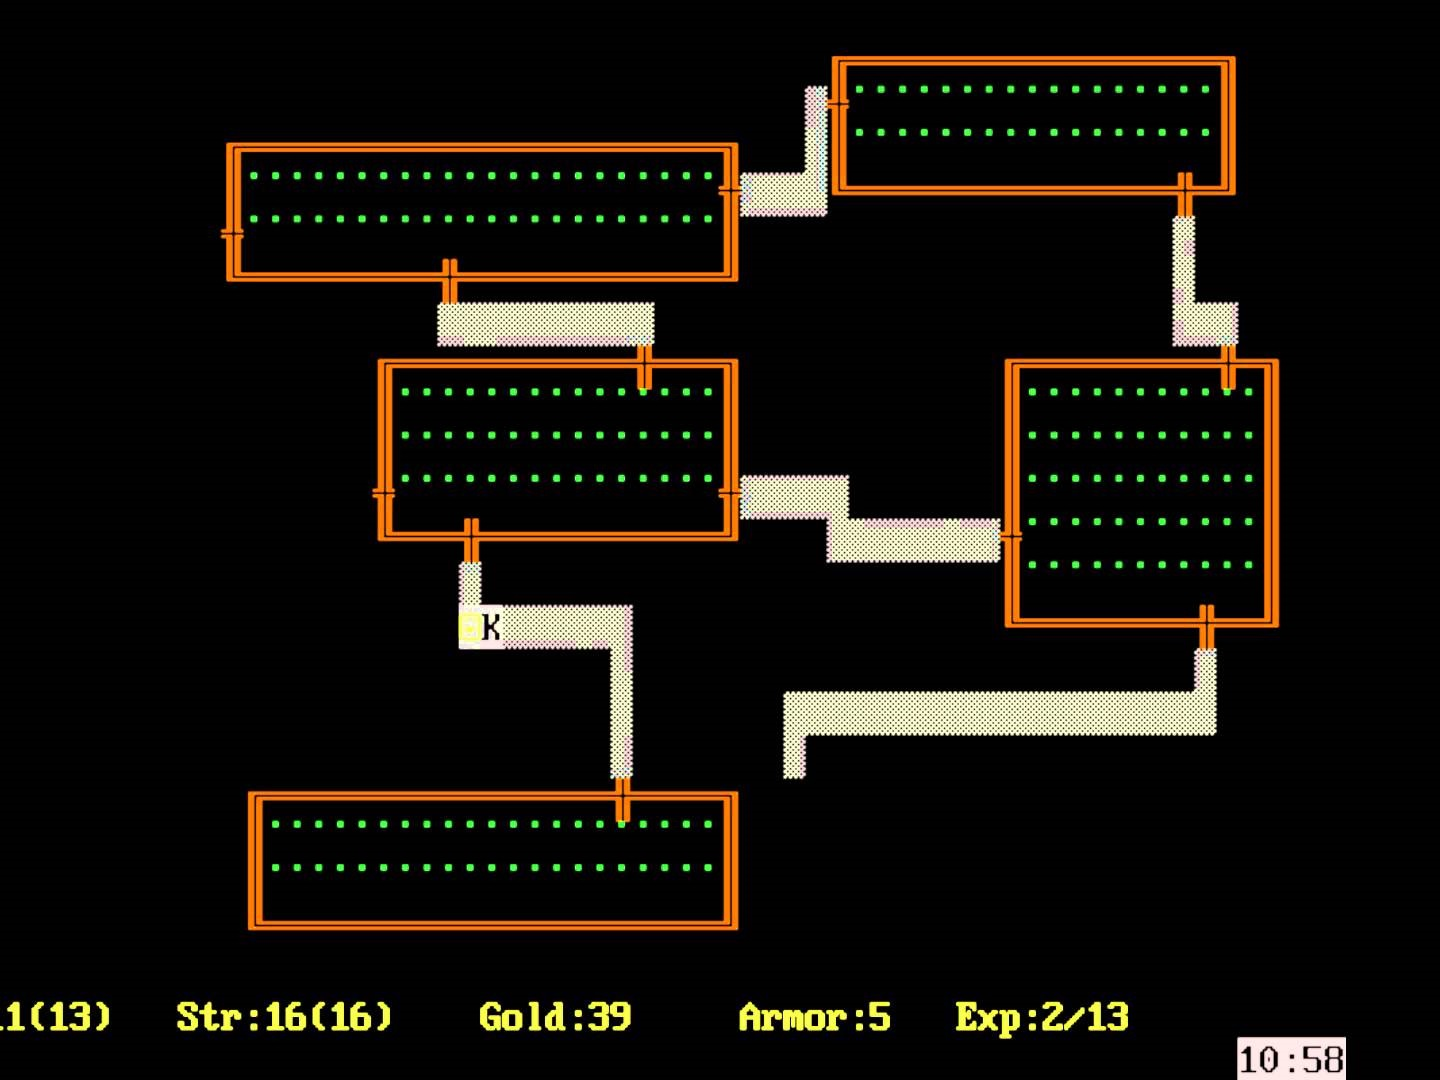
\includegraphics[width=\paperwidth]{img/games/rogue.jpg}}
\begin{frame}[plain]
\end{frame}

\usebackgroundtemplate{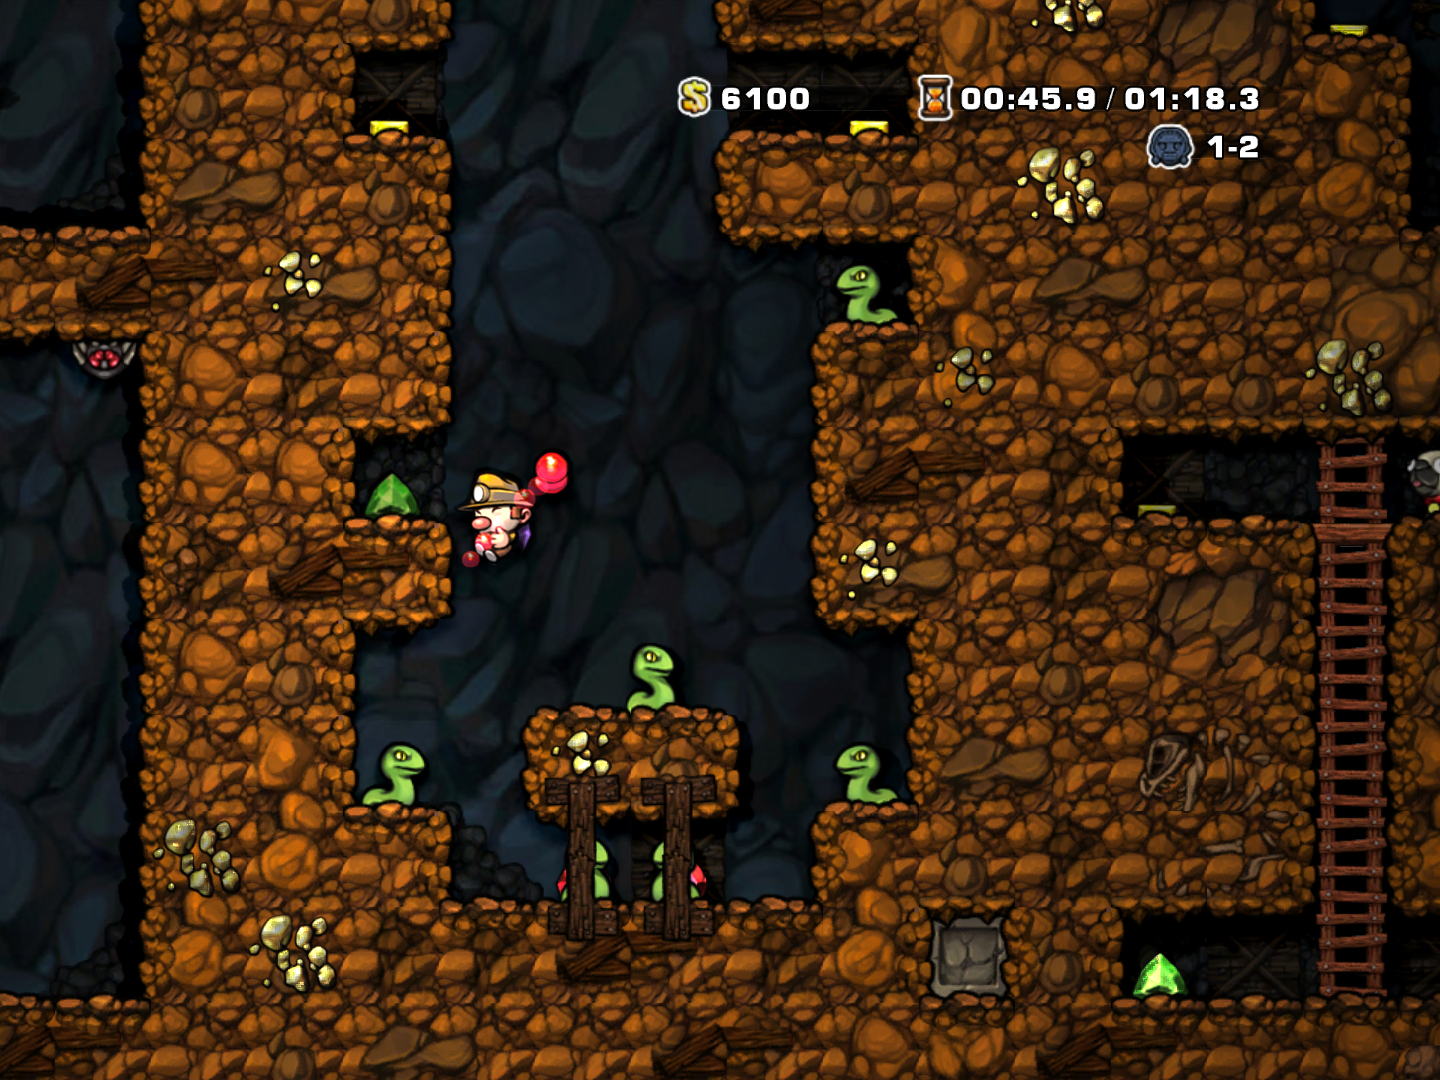
\includegraphics[width=\paperwidth]{img/games/spelunky.png}}
\begin{frame}[plain]
\end{frame}

\usebackgroundtemplate{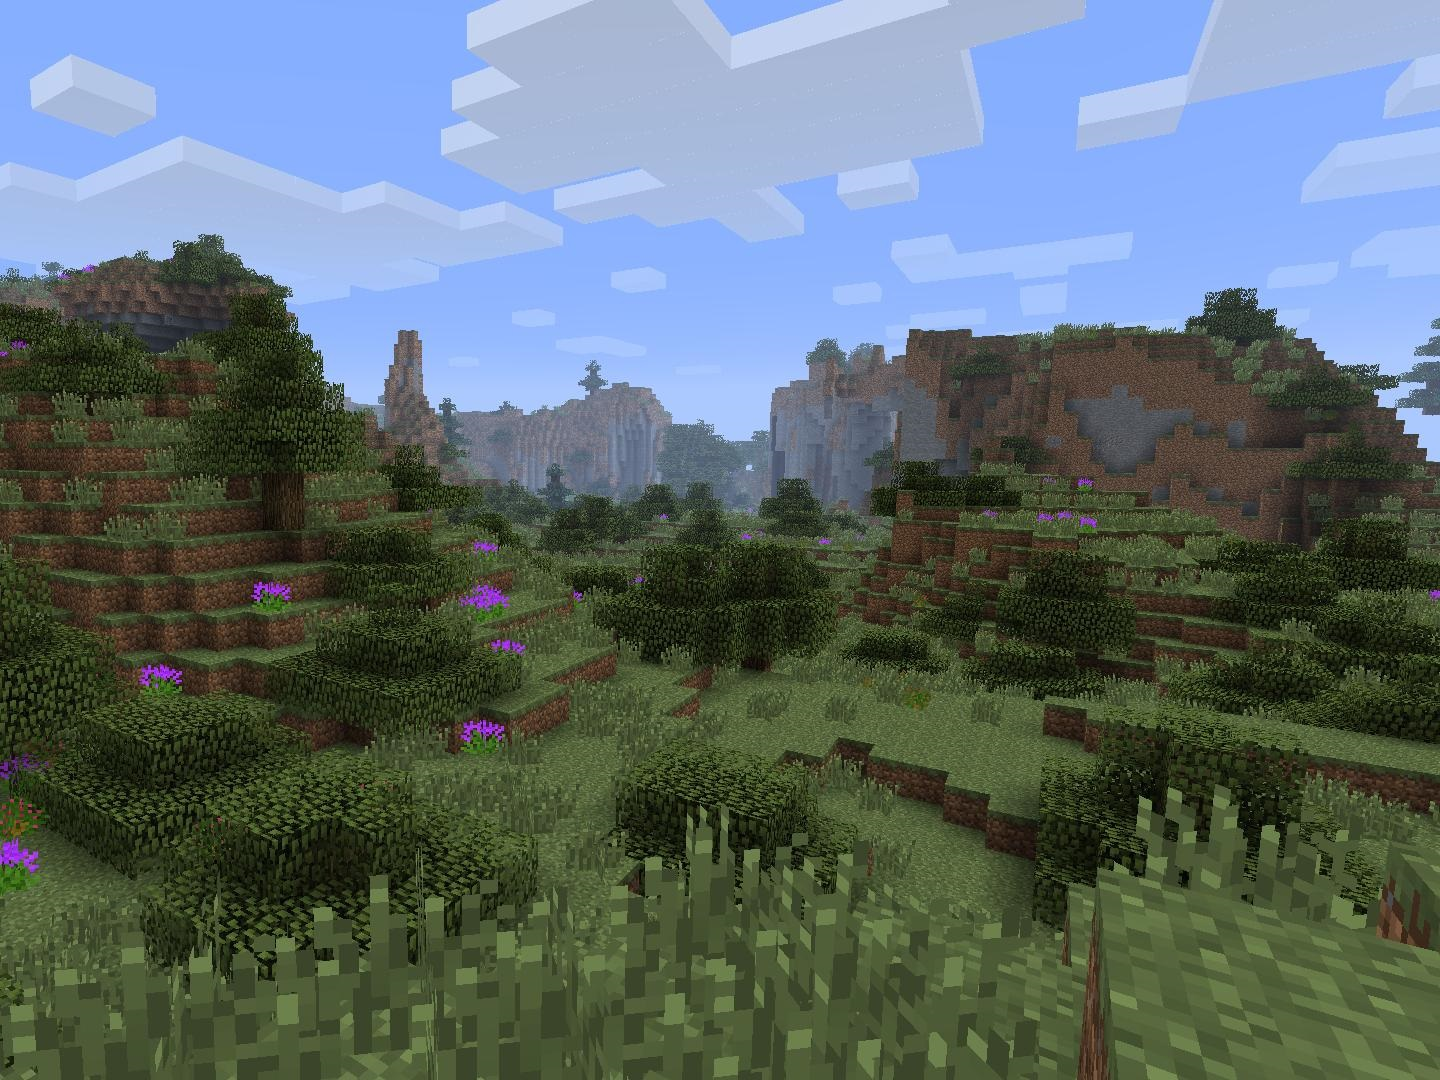
\includegraphics[width=\paperwidth]{img/games/minecraft.jpg}}
\begin{frame}[plain]
\end{frame}

\usebackgroundtemplate{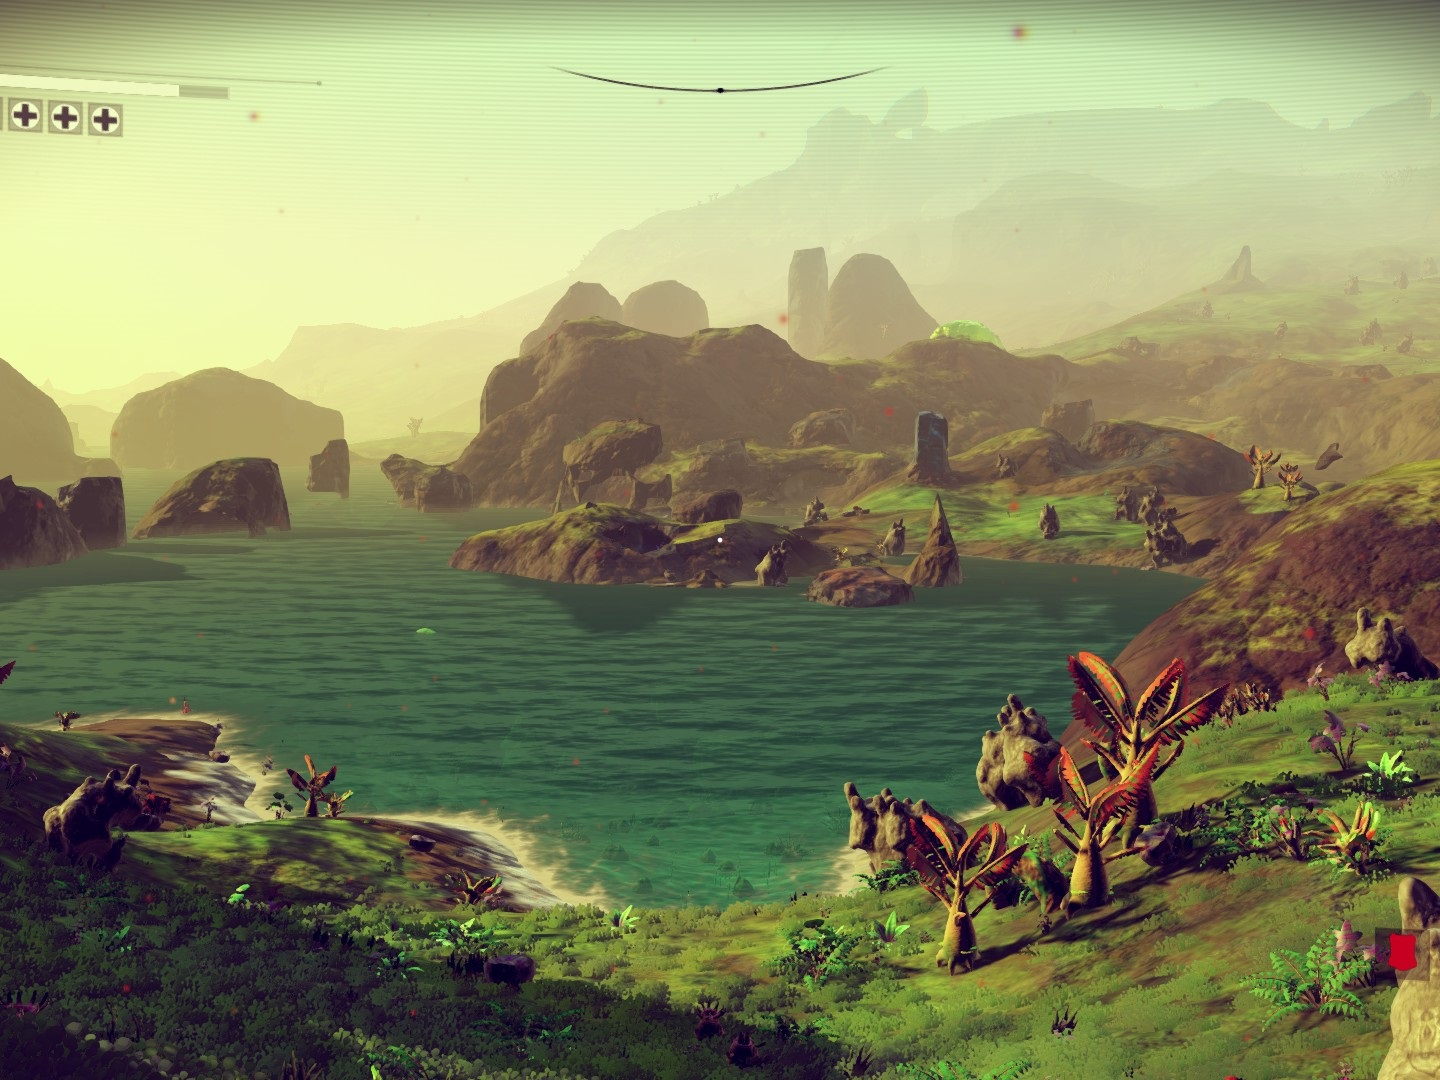
\includegraphics[width=\paperwidth]{img/games/nms1.jpg}}
\begin{frame}[plain]
\end{frame}

\usebackgroundtemplate{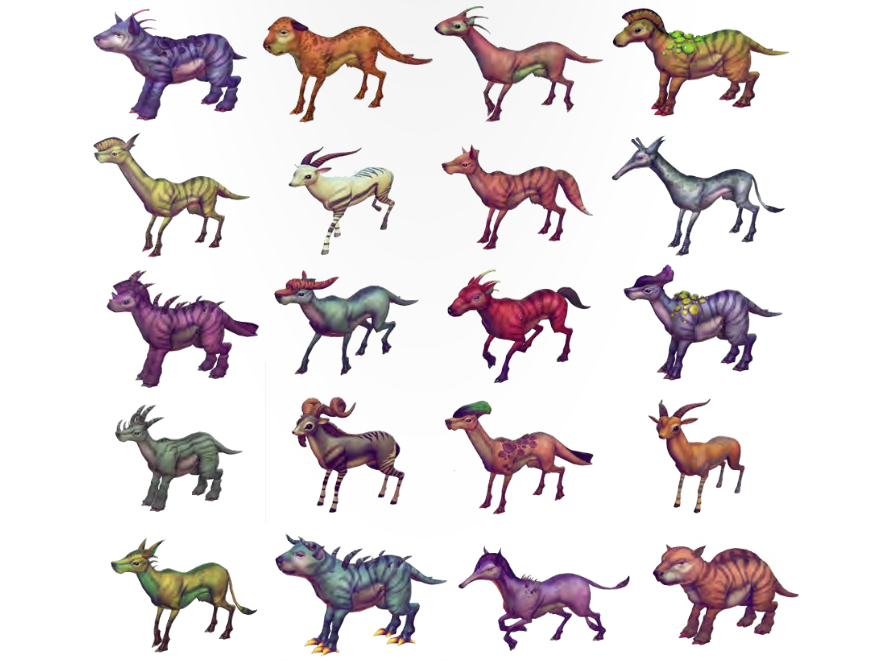
\includegraphics[width=\paperwidth]{img/games/nms2.png}}
\begin{frame}[plain]
\end{frame}

\usebackgroundtemplate{}

\begin{frame}
	\begin{columns}[c]
		\column{.3\textwidth}
		\centering		
		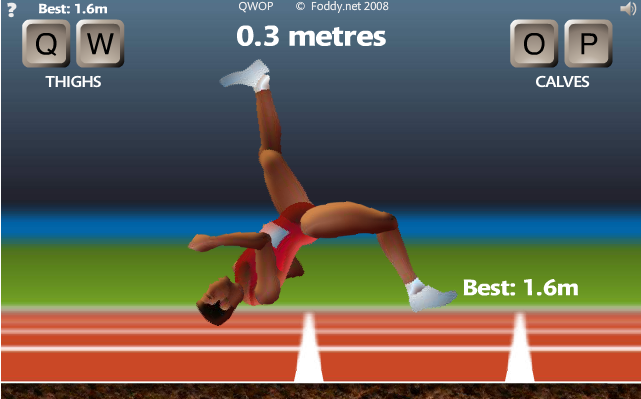
\includegraphics[width=\textwidth]{img/games/qwop.png} \\
		\vspace{1.5em}
		\textbf{Bewegungssteurung}
		\column{.1\textwidth}
		\centering
		\textbf{\huge +}
		\column{0.2\textwidth}
		\centering
		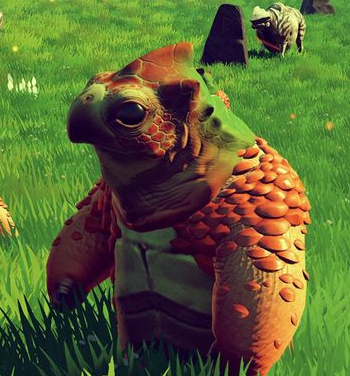
\includegraphics[width=\textwidth]{img/games/nms3.png} \\
		\vspace{1.5em}
		\textbf{Prozedurale Kreaturen}
		\column{.1\textwidth}
		\centering
		\textbf{\huge =}
		\column{.3\textwidth}
		\centering
		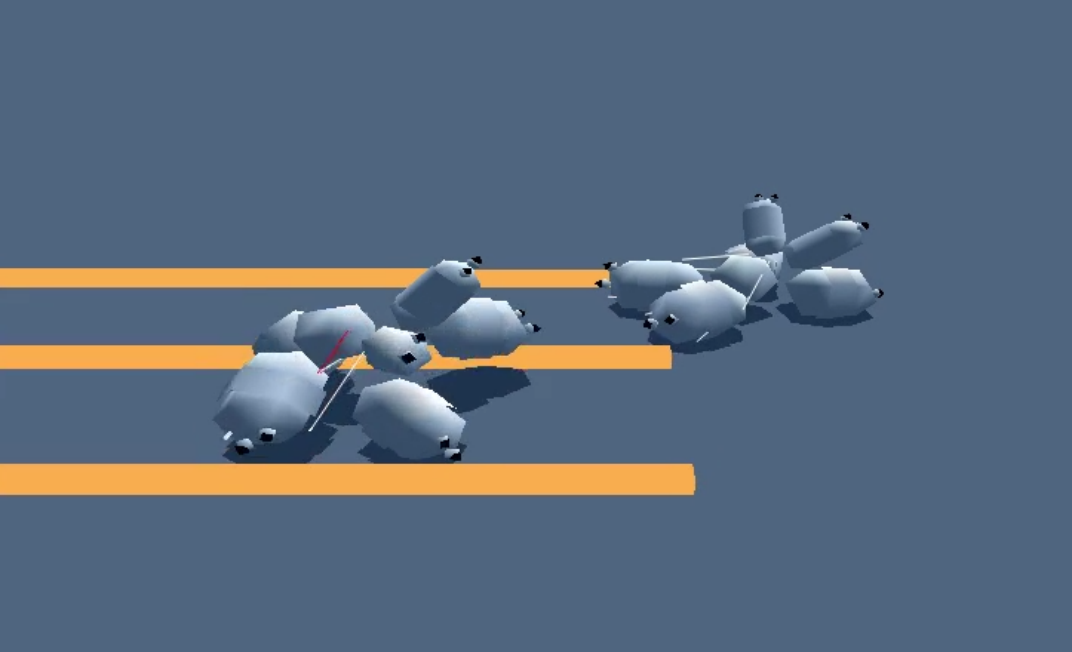
\includegraphics[width=\textwidth]{img/games/darwin.png} \\
		\vspace{1.5em}
		\textbf{Darwin's Avatars}
	\end{columns}
	
\end{frame}

\usebackgroundtemplate{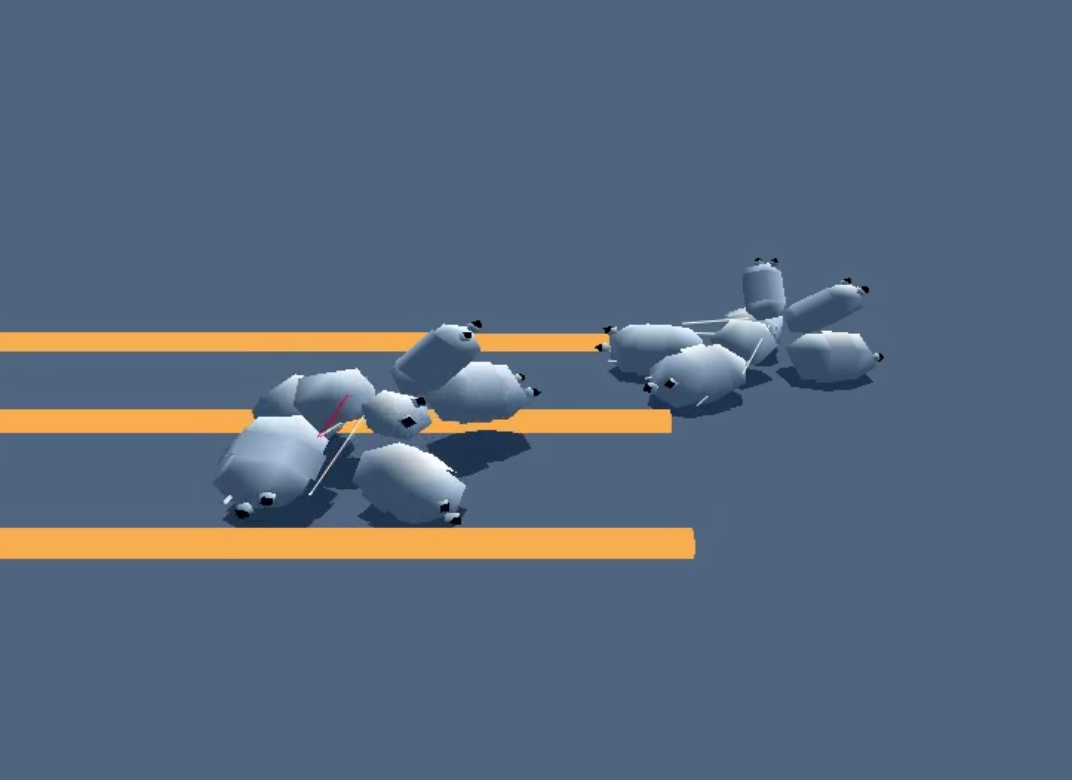
\includegraphics[width=\paperwidth]{img/games/darwin2.png}}

\begin{frame}
	\frametitle{Darwin's Avatars}	
\end{frame}

\usebackgroundtemplate{}

\begin{frame}
	\frametitle{Darwin's Avatars}
	\textbf{Vorgehensweise}\\ \pause
	\begin{itemize}
		\item Entwickle Körper und Gehirn evolutionär \pause
		\begin{itemize}
			\item Fitness = Spielziel \pause
		\end{itemize} 
		\item Entferne Gehirn \pause
		\item Spieler steuert die Kreatur \pause
		\item Messe Zeit bzw. Geschwindigkeit
	\end{itemize}	
\end{frame}

\begin{frame}
	\frametitle{Kodierung von Evolved Virtual Creatures (EVCs)}
	\begin{columns}[c]
		\column{.4\textwidth}
		\centering
		\resizebox{0.8\textwidth}{!}{
			\begin{tikzpicture}[->,shorten >=1pt,auto,node distance=0.7cm,main node/.style={circle,draw,font=\sffamily\Large\bfseries}]
			
			\node[main node] (1) {};
			\node[main node] (2) [below left of = 1] {};
			\node[main node] (3) [below right of = 1] {};
			
			\path[every node/.style={font=\sffamily\small}]
			(1) edge [bend right] node[left] {} (2)
				edge [bend left] node[left] {} (3)			
			;
			\end{tikzpicture}
		}
		\column{.6\textwidth}
		\centering
		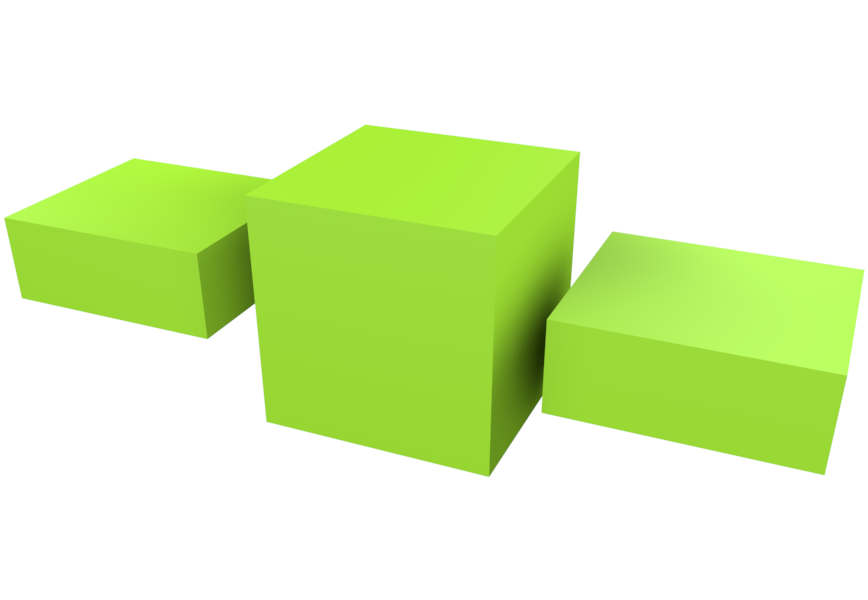
\includegraphics[width=\textwidth]{img/1.png}
	\end{columns}
\end{frame}

\begin{frame}[noframenumbering]
	\frametitle{Kodierung von Evolved Virtual Creatures (EVCs)}
	\begin{columns}[c]
		\column{.4\textwidth}
		\centering
		\resizebox{0.4\textwidth}{!}{
			\begin{tikzpicture}[->,shorten >=1pt,auto,node distance=0.85cm,main node/.style={circle,draw,font=\sffamily\Large\bfseries}]
			
			\node[main node] (1) {};
			\node[main node] (2) [below of = 1] {};
			
			\path[every node/.style={font=\sffamily\small}]
			(1) edge [bend right = 20] node[left] {} (2)
				edge [bend left = 20] node[left] {} (2)			
			;
			\end{tikzpicture}
		}
		\column{.6\textwidth}
		\centering
		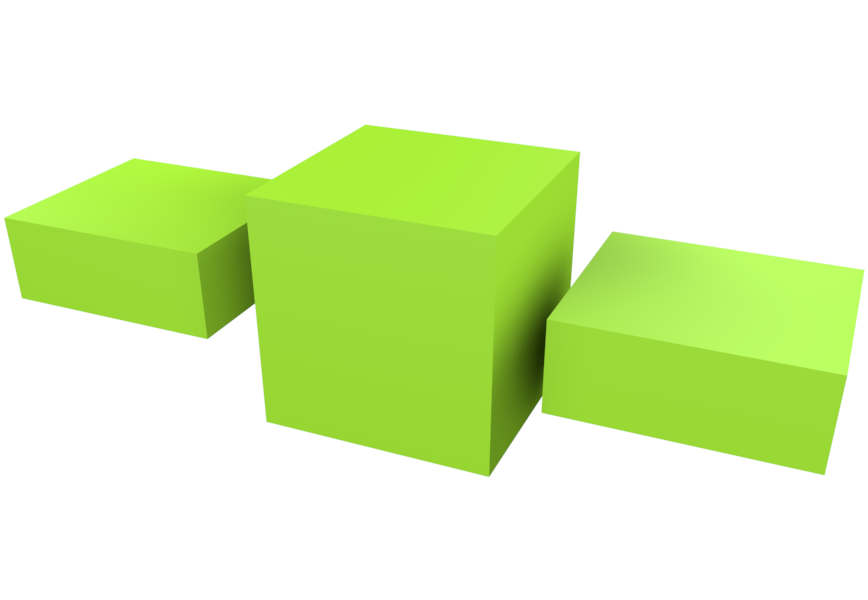
\includegraphics[width=\textwidth]{img/1.png}
	\end{columns}
\end{frame}

\begin{frame}
	\frametitle{Kodierung von Evolved Virtual Creatures (EVCs)}
	\begin{columns}[c]
		\column{.4\textwidth}
		\centering
		\resizebox{0.5\textwidth}{!}{
			\begin{tikzpicture}[->,shorten >=1pt,auto,node distance=3cm,main node/.style={circle,draw,font=\sffamily\Large\bfseries}]
			
			\node[main node] (1) {};
			\draw (1) to [out=60,in=120,looseness=8, min distance=0.5cm] (1);
			\end{tikzpicture}
		}
		
		\column{.6\textwidth}
		\centering
		
\includegraphics[width=0.8\textwidth]{img/2.png}
	\end{columns}
\end{frame}

\begin{frame}
	\frametitle{Kodierung von Evolved Virtual Creatures (EVCs)}
	\begin{columns}[c]
		\column{.4\textwidth}
		\centering
		\resizebox{0.8\textwidth}{!}{
			\begin{tikzpicture}[->,shorten >=1pt,auto,node distance=10cm,main node/.style={circle,draw,font=\sffamily\Large\bfseries}]
			
			\node[main node] (1) {};
			
			\draw (1) to [out=165,in=105,looseness=8, min distance=0.5cm] (1);
			\draw (1) to [out=15,in=75,looseness=8, min distance=0.5cm] (1);
			\end{tikzpicture}
		}
		\column{.6\textwidth}
		\centering
		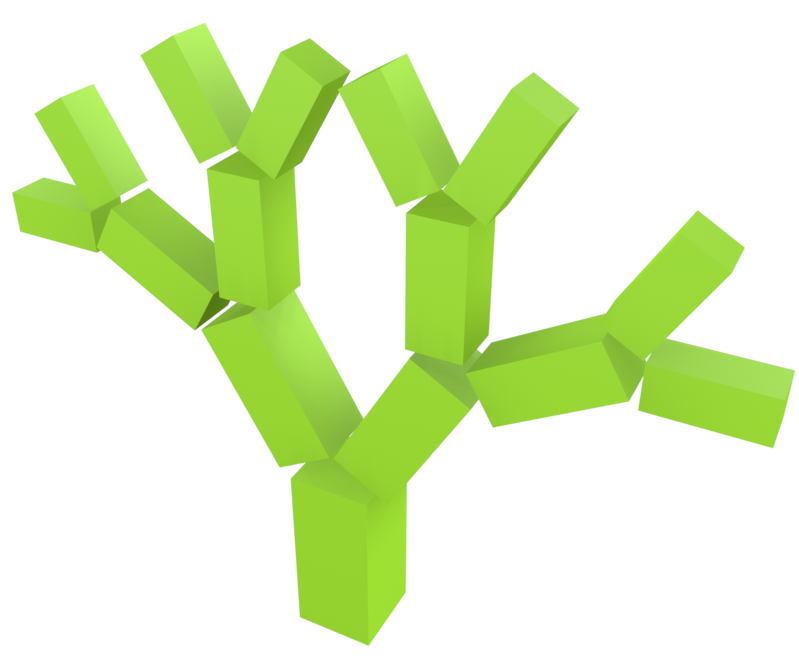
\includegraphics[width=\textwidth]{img/3.png}
	\end{columns}
\end{frame}

\begin{frame}
	\frametitle{Kodierung von Evolved Virtual Creatures (EVCs)}
	\begin{columns}[c]
		\column{.4\textwidth}
		\centering
		\resizebox{0.5\textwidth}{!}{
			\begin{tikzpicture}[->,shorten >=1pt,auto,node distance=1cm,main node/.style={circle,draw,font=\sffamily\Large\bfseries}]
			
			\node[main node] (1) {};
			\node[main node] (2) [below of = 1] {};
			
			\draw (1) to [out=60,in=120,looseness=8, min distance=0.5cm] (1);
			\draw (2) to [out=300,in=240,looseness=8, min distance=0.5cm] (2);
			
			\path[every node/.style={font=\sffamily\small}]
			(1) edge [bend right = 20] node[left] {} (2)
				edge [bend left = 20] node[left] {} (2)			
			;
			\end{tikzpicture}
		}
		\column{.6\textwidth}
		\centering
		
\includegraphics[width=\textwidth]{img/4.png}
	\end{columns}
\end{frame}

\begin{frame}[noframenumbering]
	\frametitle{Kodierung von Evolved Virtual Creatures (EVCs)}
	\begin{columns}[c]
		\column{.4\textwidth}
		\centering
		\resizebox{0.5\textwidth}{!}{
			\begin{tikzpicture}[->,shorten >=1pt,auto,node distance=0.8cm,main node/.style={circle,draw,font=\sffamily\Large\bfseries}]
			
			\node[main node] (1) {};
			\node[main node] (2) [below of = 1] {};
			\node[main node] (3) [above of = 1] {};
			
			\draw (2) to [out=300,in=240,looseness=8, min distance=0.5cm] (2);
			
			\draw (1) to [] (3);
			
			\path[every node/.style={font=\sffamily\small}]
			(1) edge [bend right = 10] node[left] {} (2)
			edge [bend left = 10] node[left] {} (2)
			edge [bend right = 30] node[left] {} (2)
			edge [bend left = 30] node[left] {} (2)
			;
			\end{tikzpicture}
		}
		\column{.6\textwidth}
		\centering
		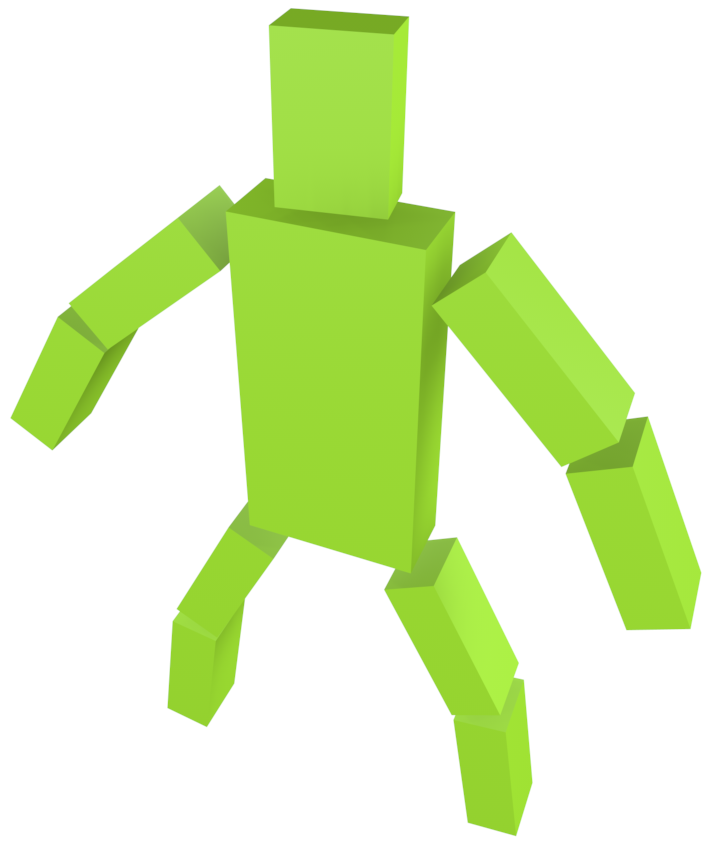
\includegraphics[width=0.8\textwidth]{img/5.png}
	\end{columns}
\end{frame}

%Beginn meiner Folien

\begin{frame}
	\frametitle{Kontrolle der Kreaturen}
	\textbf{Bestandteile}\\ \pause
	\begin{itemize}
		\item Propriozeptoren arbeiten wie Sensoren \pause
		\begin{itemize}
			\item Aktuelle Länge von jedem Muskel wird gemessen \pause
			\item Weitere Sensoren möglich, aber nicht im Spiel enthalten \pause
		\end{itemize}
		\item Neuronen können Funktionen auf ein Eingangssignal anwenden \pause
		\begin{itemize}
			\item Beispiele sind Summe, Produkt, Sinus, boolische Operationen \pause
		\end{itemize}
		\item Effektoren erhalten einen Wert und führen davon abhängig eine Bewegung aus
		\item Jeder dieser Bausteine wird im Graphen in Form eines Knoten dargestellt
	\end{itemize}
\end{frame}

\begin{frame}
	\frametitle{Erweiterter Graph einer Kreatur}
	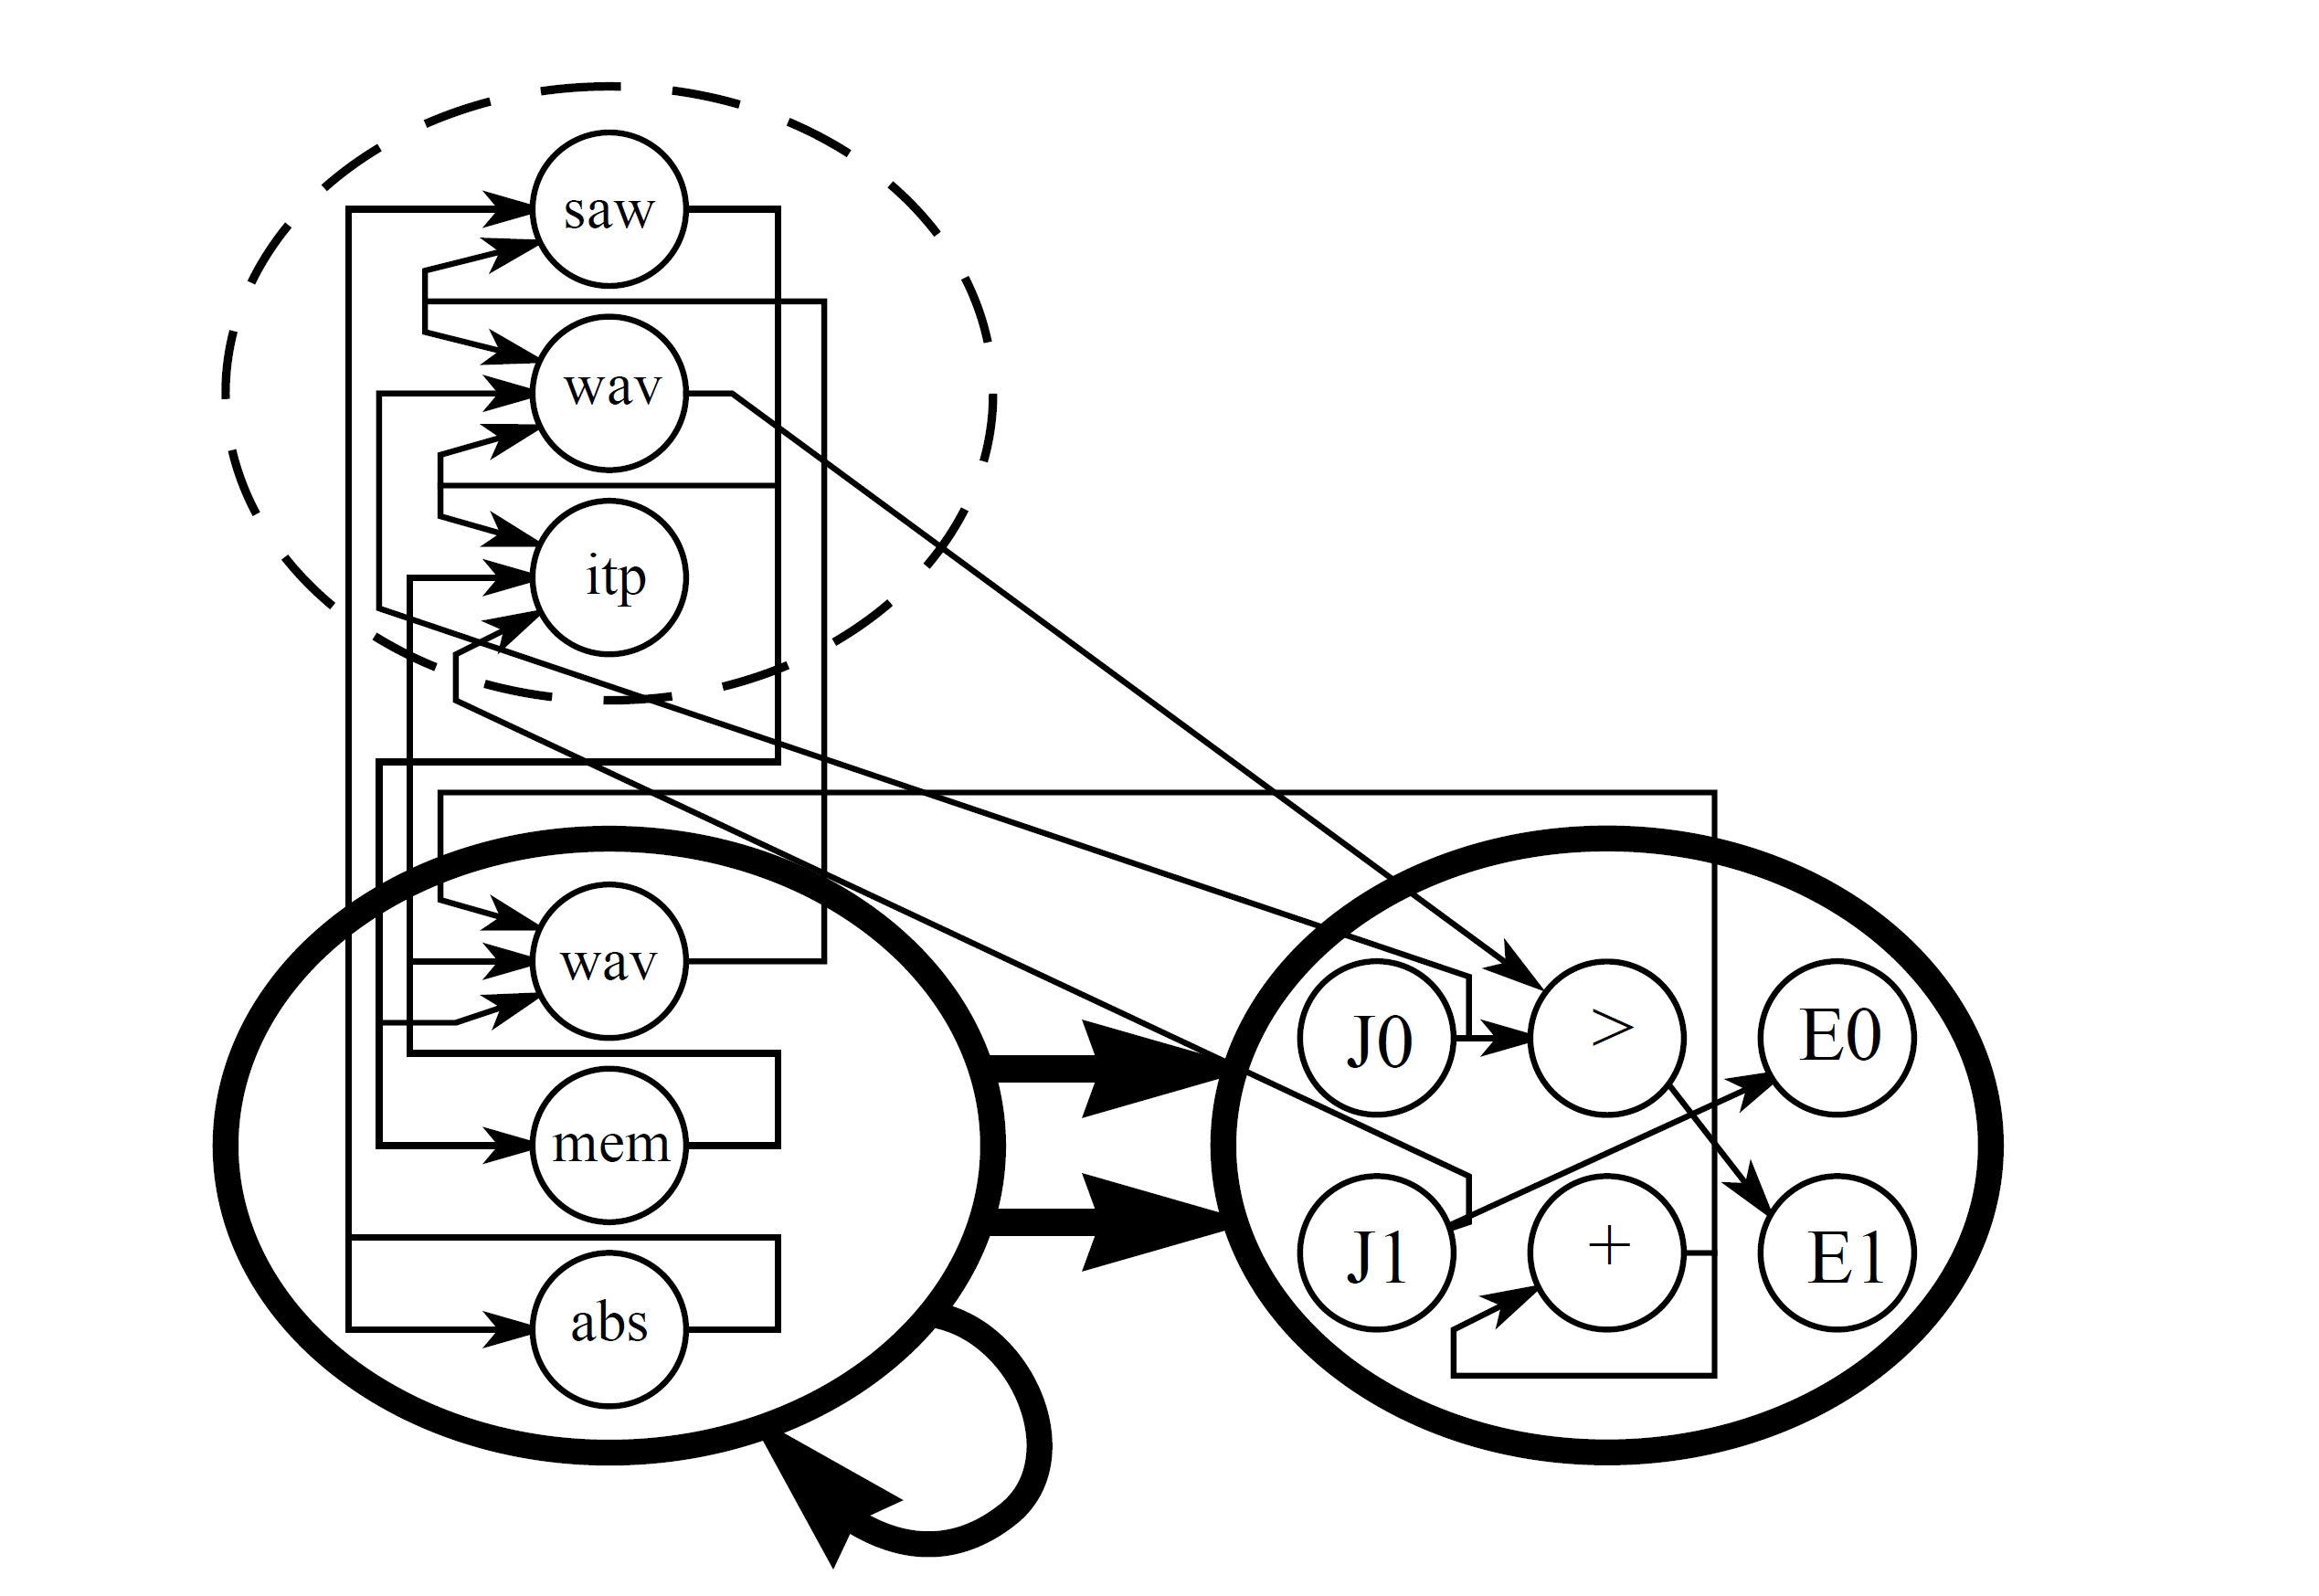
\includegraphics[width=0.9\textwidth]{img/evolved_graph.png} 
\end{frame}

\begin{frame}
	\frametitle{Entstandene Kreatur und das zugehörige Gehirn}
	\begin{columns}
		\column{.4\textwidth}
		\centering
		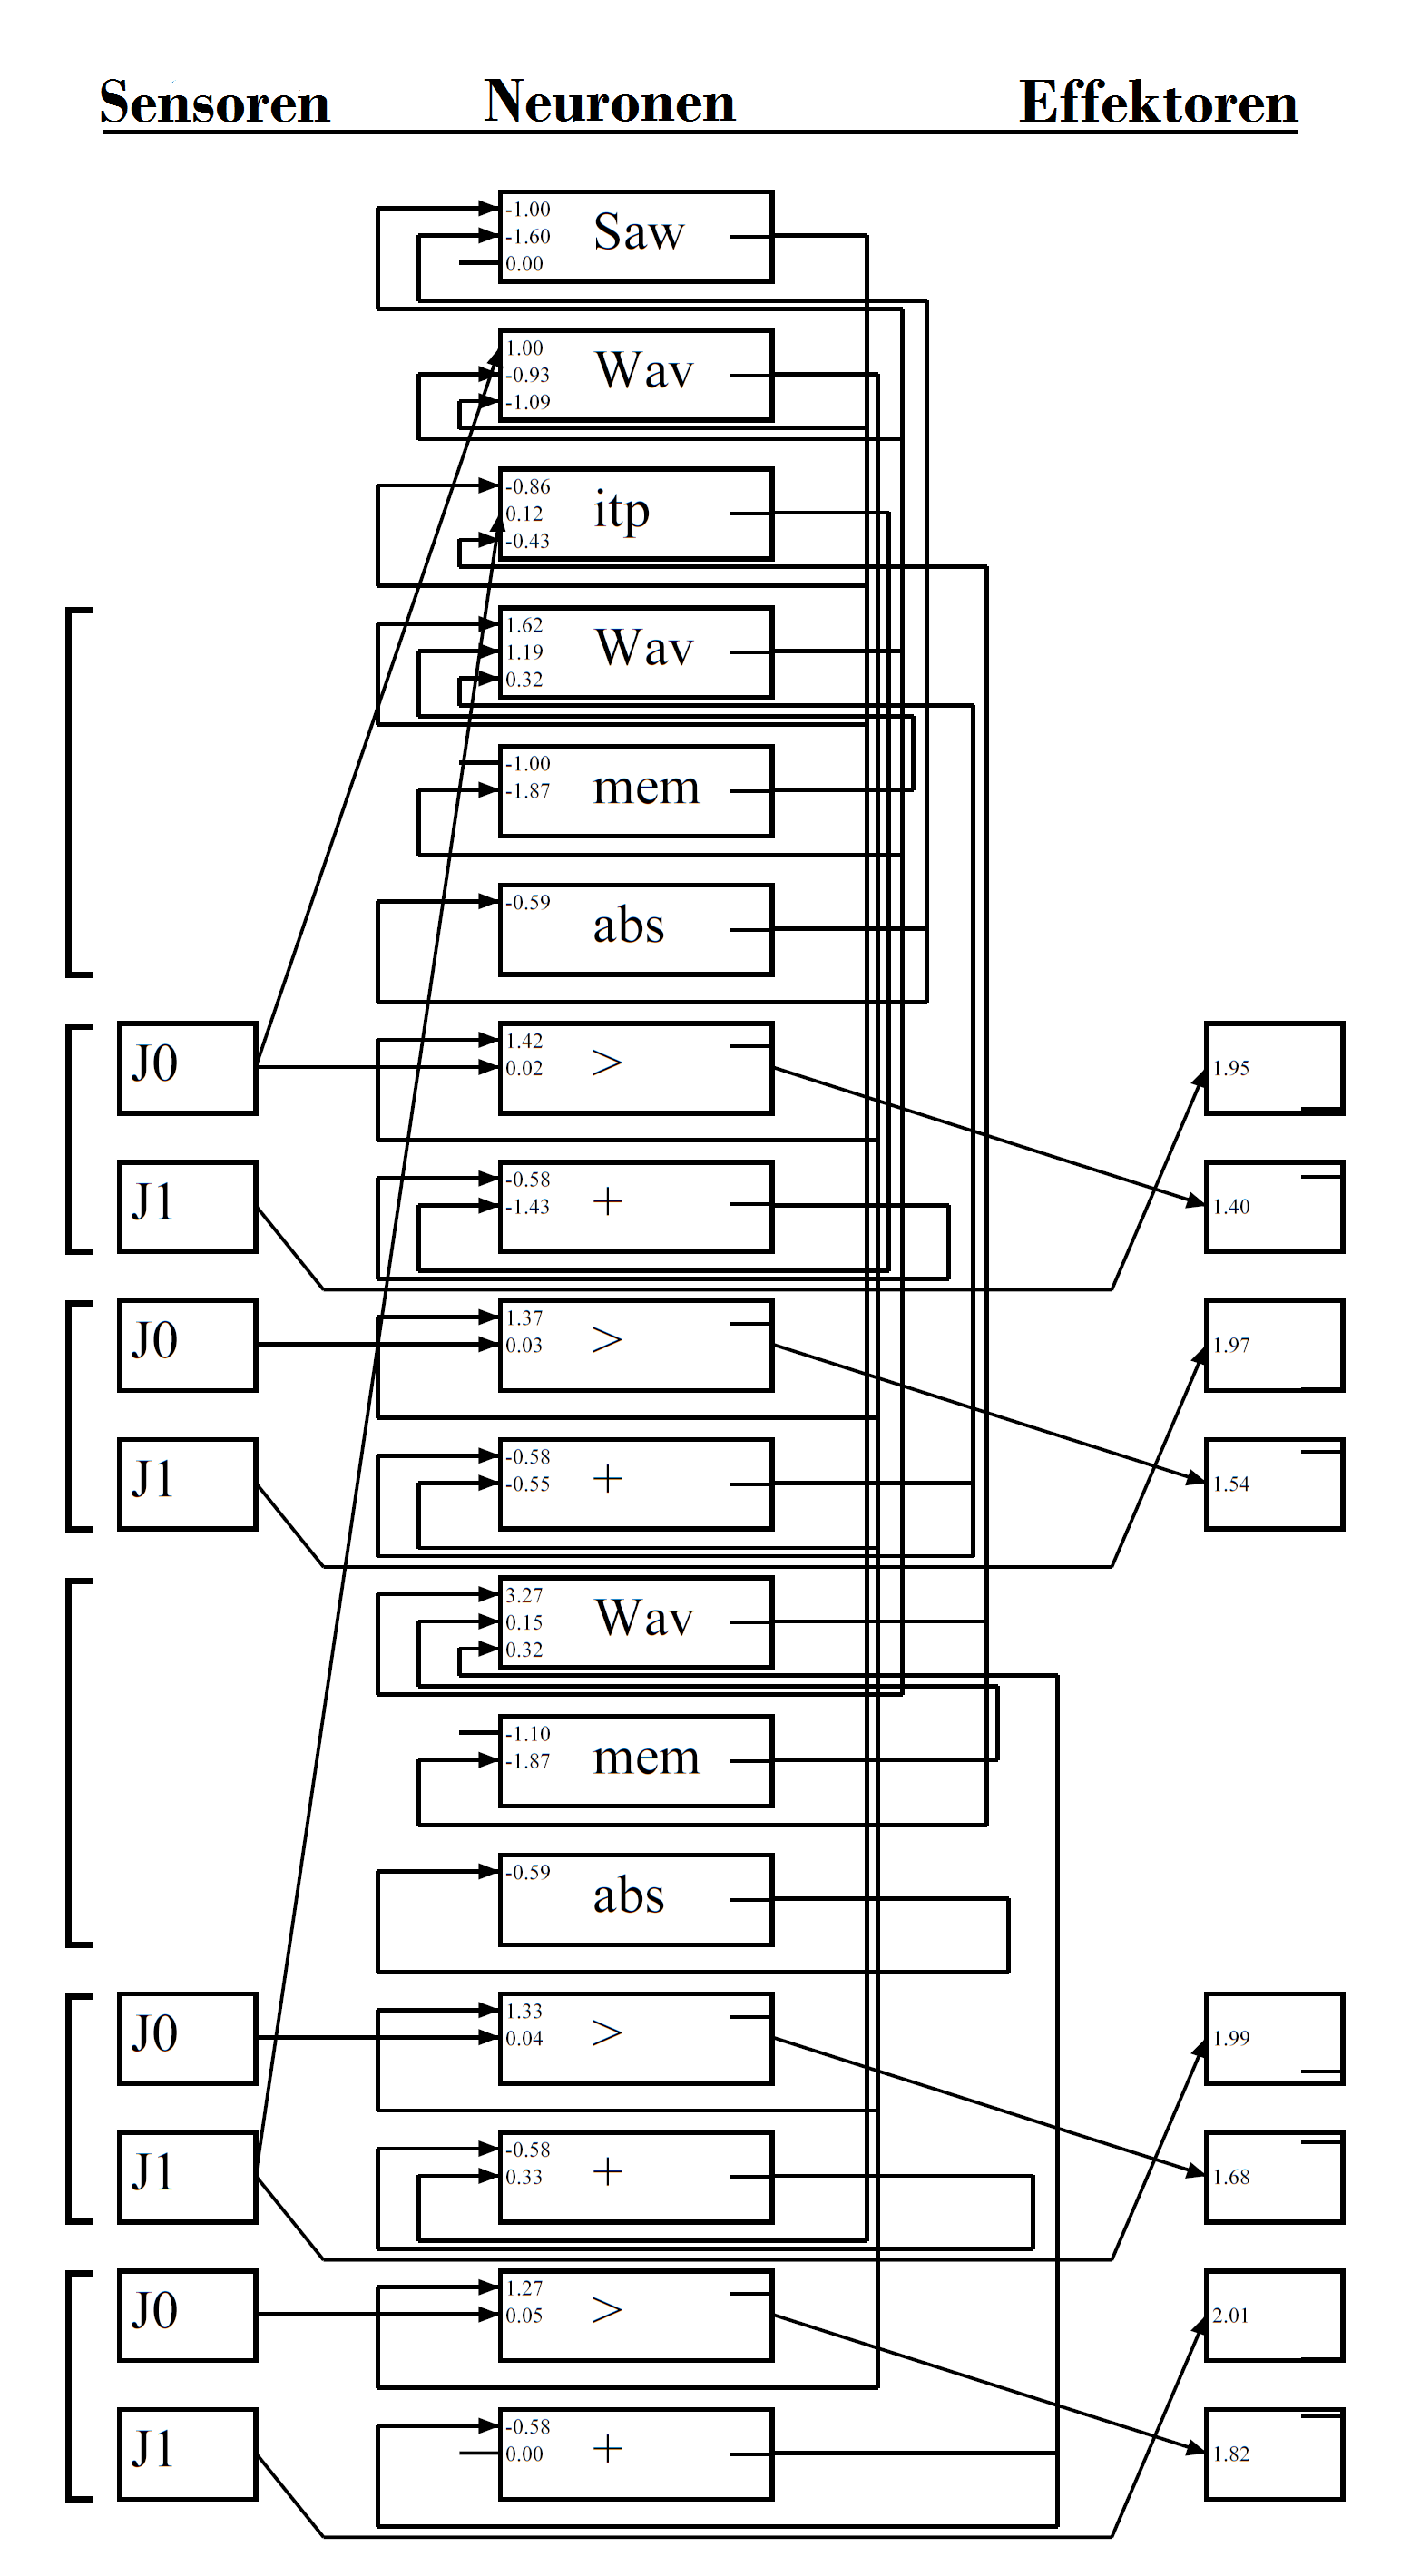
\includegraphics[width=0.9\textwidth]{img/brain(1).png} \pause
		\column{.2\textwidth}
		\centering
		$\longrightarrow$
		\column{.4\textwidth}
		\centering
		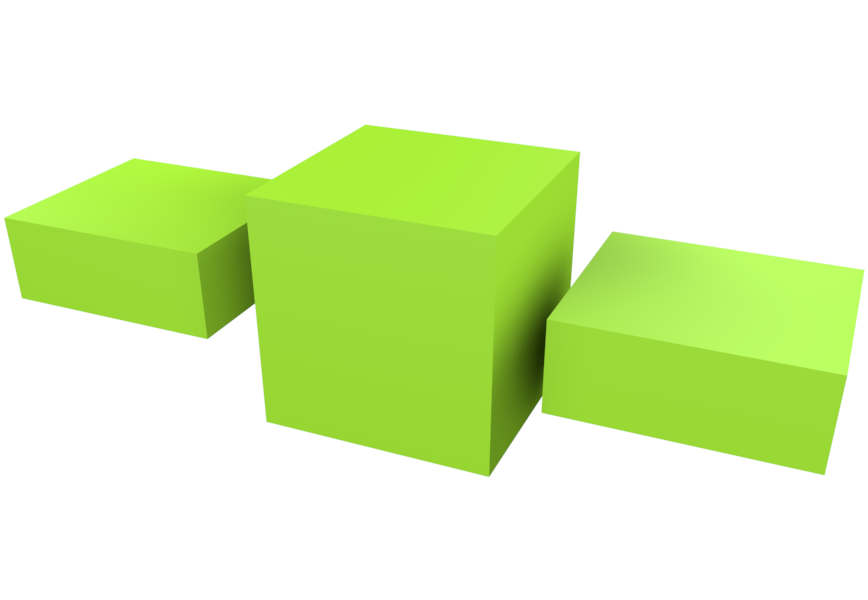
\includegraphics[width=\textwidth]{img/1.png}
	\end{columns}
\end{frame}

\begin{frame}
	\frametitle{Messergebnisse (1/6)}
	\begin{columns}
		\column{.5\textwidth}
		\begin{figure}
			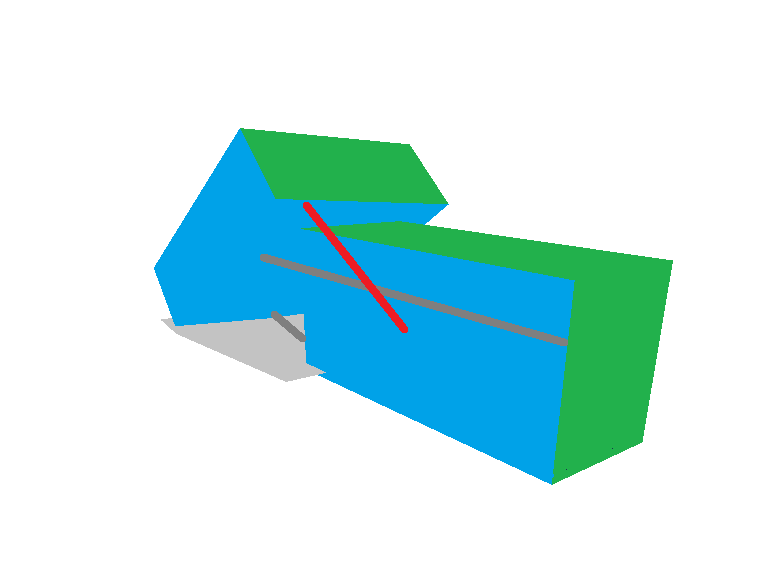
\includegraphics[width=0.68\textwidth]{img/type1.png} \pause
		\end{figure}
		\begin{figure}
			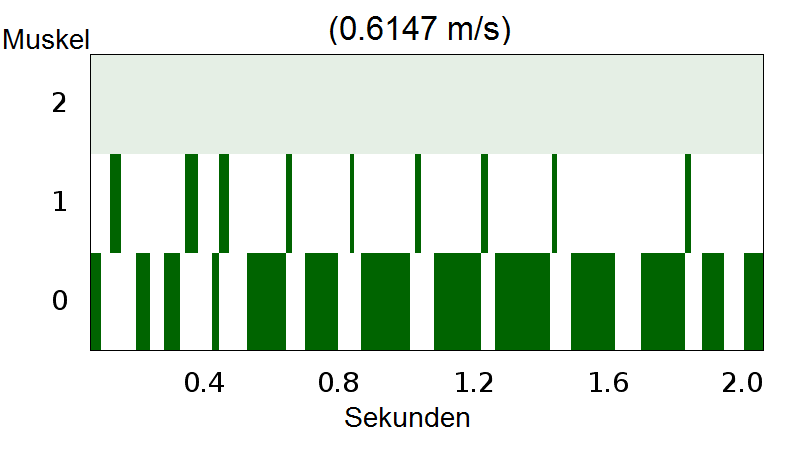
\includegraphics[width=0.9\textwidth]{img/hum12.png}
		\end{figure}
		\column{.5\textwidth}
		\begin{figure}
			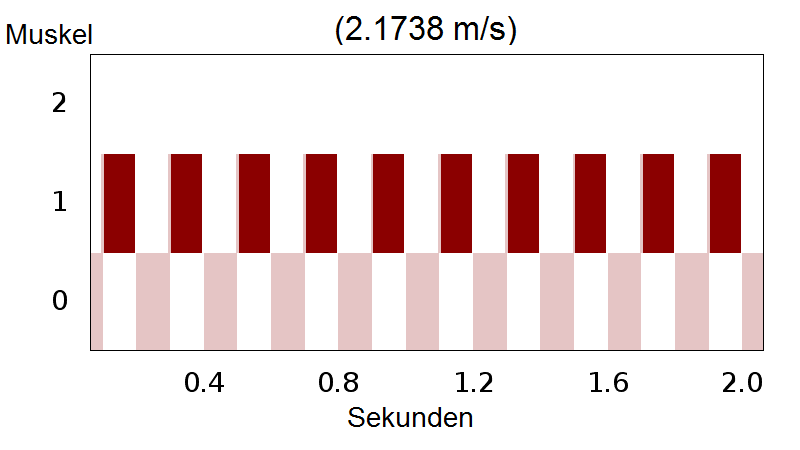
\includegraphics[width=0.9\textwidth]{img/ki1.png} 
		\end{figure}
		\begin{figure}
			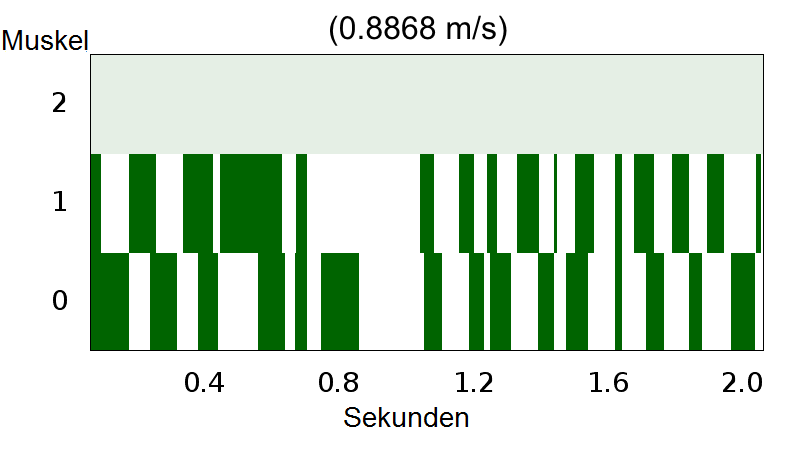
\includegraphics[width=0.9\textwidth]{img/hum11.png}
		\end{figure}
	\end{columns}
\end{frame}

\begin{frame}
	\frametitle{Messergebnisse (2/6)}
	\begin{columns}
		\column{.5\textwidth}
		\begin{figure}
			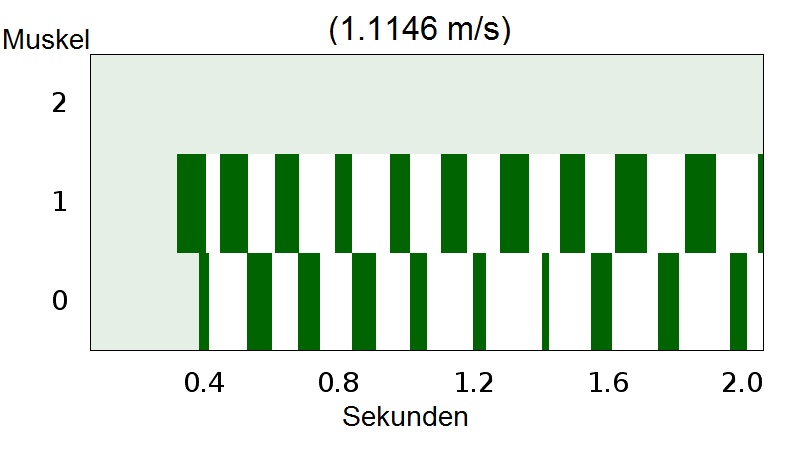
\includegraphics[width=0.9\textwidth]{img/hum13.png} 
		\end{figure}
		\begin{figure}
			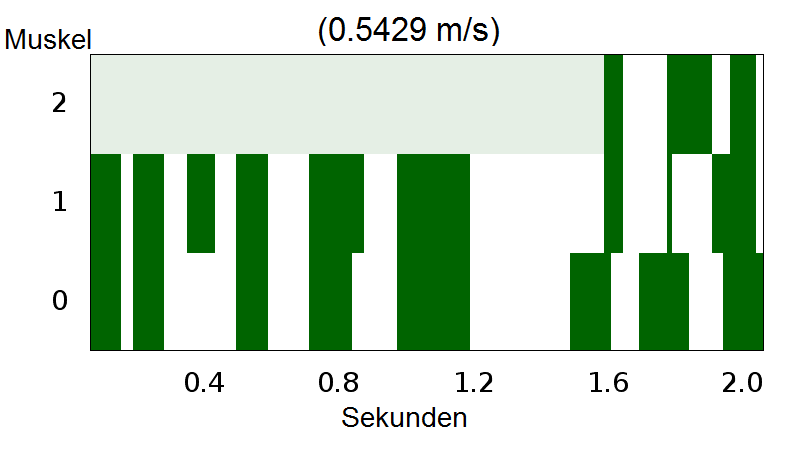
\includegraphics[width=0.9\textwidth]{img/hum15.png}
		\end{figure}
		\column{.5\textwidth}
		\begin{figure}
			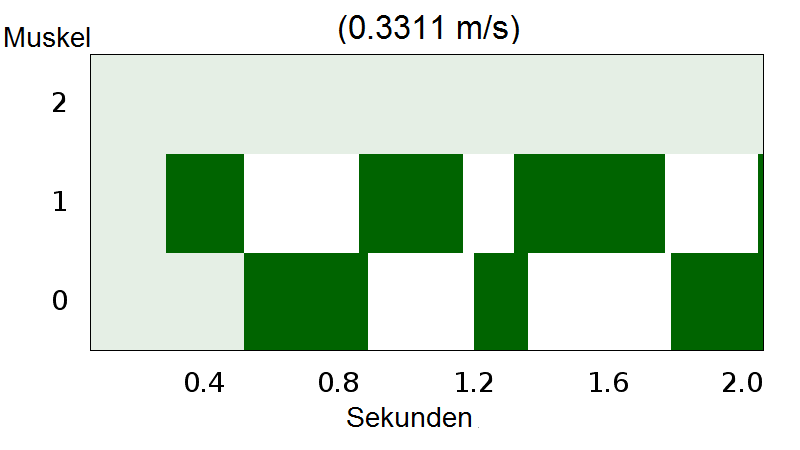
\includegraphics[width=0.9\textwidth]{img/hum14.png} 
		\end{figure}
		\begin{figure}
			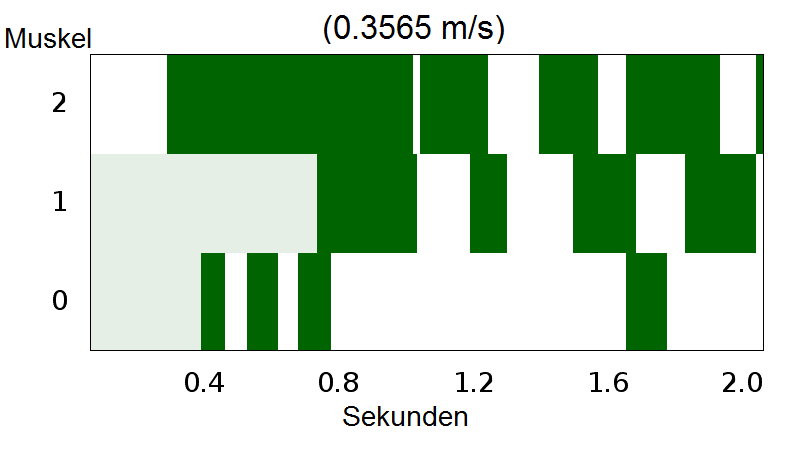
\includegraphics[width=0.9\textwidth]{img/hum16.png}
		\end{figure}
	\end{columns}
\end{frame}



\begin{frame}
	\frametitle{Messergebnisse (3/6)}
	\begin{columns}
		\column{.5\textwidth}
		\begin{figure}
			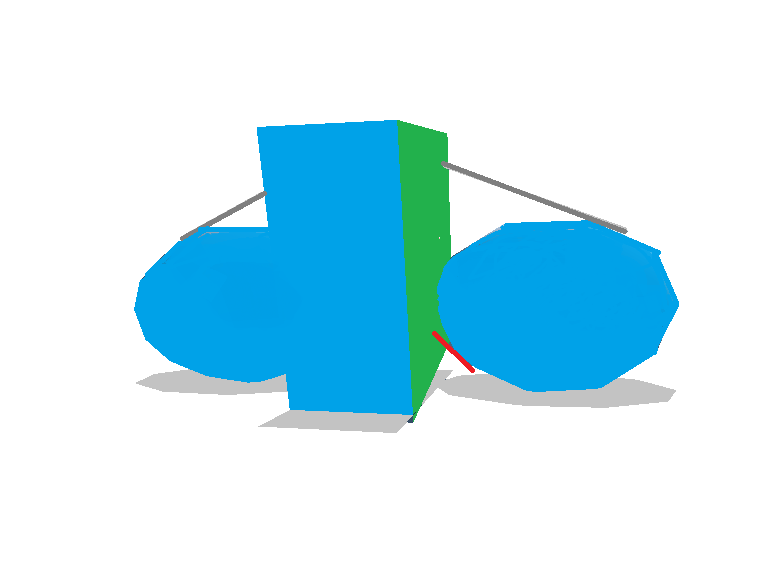
\includegraphics[width=0.68\textwidth]{img/type2.png} \pause
		\end{figure}
		\begin{figure}
			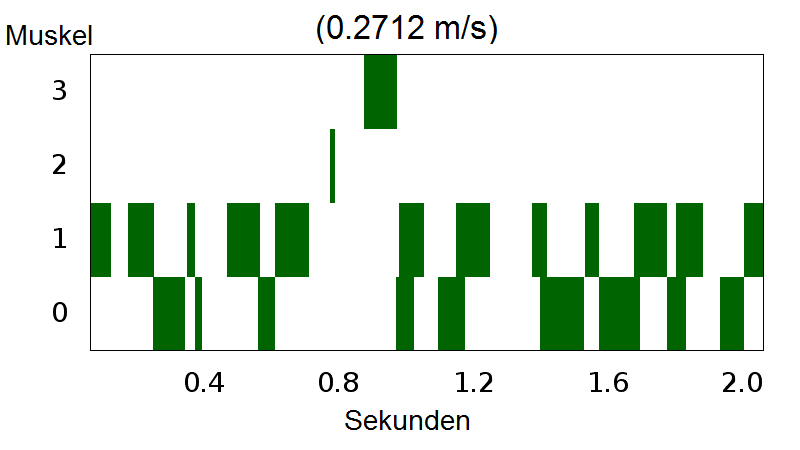
\includegraphics[width=0.9\textwidth]{img/hum22.png}
		\end{figure}
		\column{.5\textwidth}
		\begin{figure}
			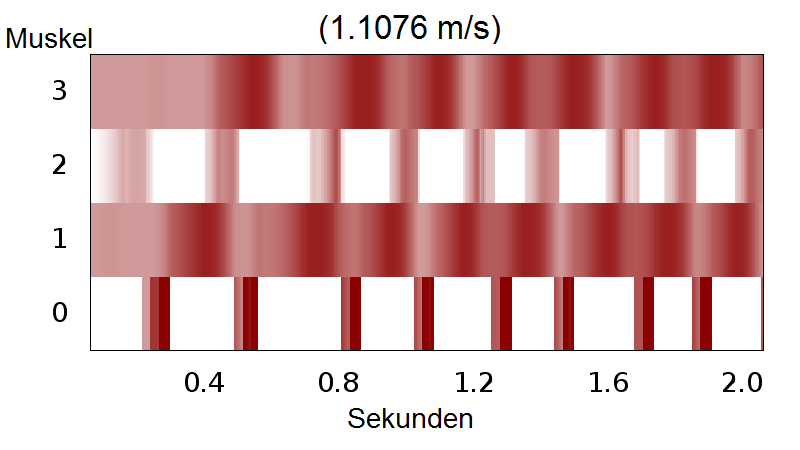
\includegraphics[width=0.9\textwidth]{img/ki2.png} 
		\end{figure}
		\begin{figure}
			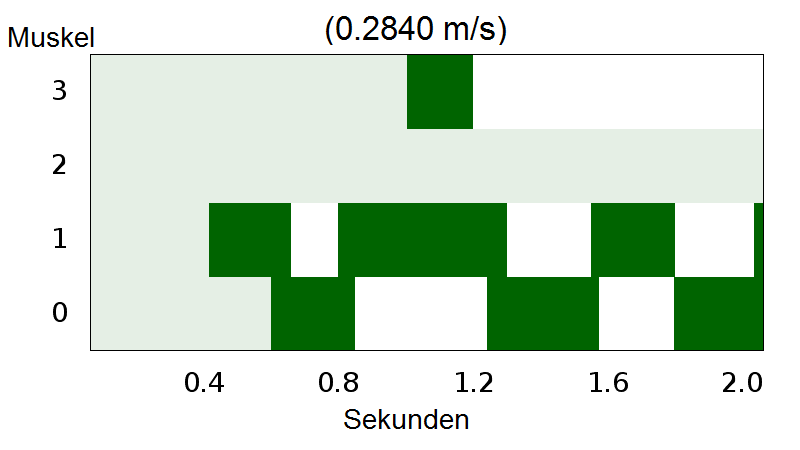
\includegraphics[width=0.9\textwidth]{img/hum21.png}
		\end{figure}
	\end{columns}
\end{frame}

\begin{frame}
	\frametitle{Messergebnisse (4/6)}
	\begin{columns}
		\column{.5\textwidth}
		\begin{figure}
			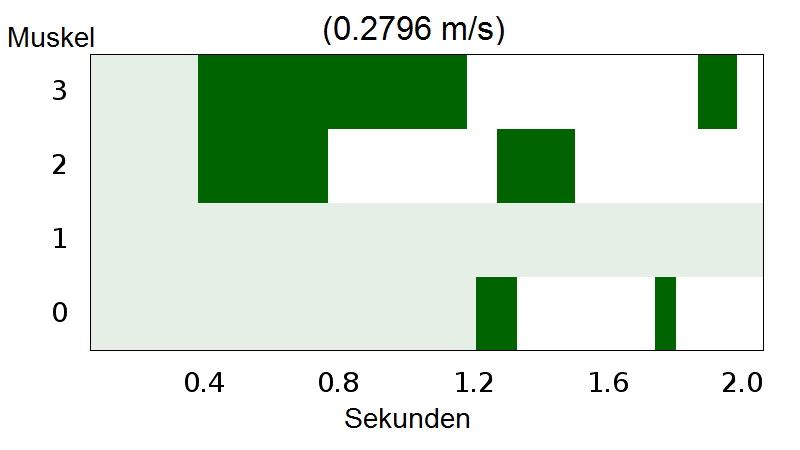
\includegraphics[width=0.9\textwidth]{img/hum23.png} 
		\end{figure}
		\begin{figure}
			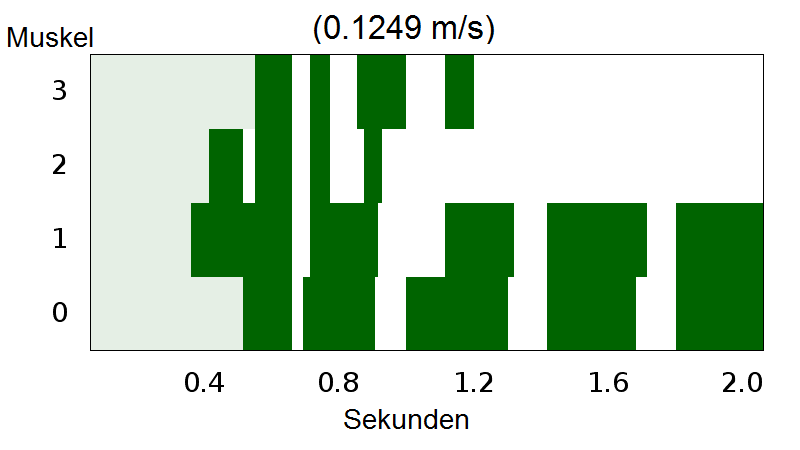
\includegraphics[width=0.9\textwidth]{img/hum25.png}
		\end{figure}
		\column{.5\textwidth}
		\begin{figure}
			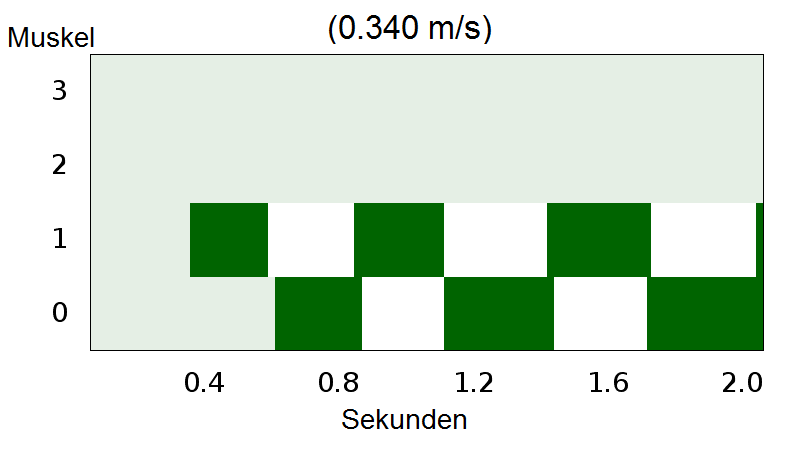
\includegraphics[width=0.9\textwidth]{img/hum24.png} 
		\end{figure}
		\begin{figure}
			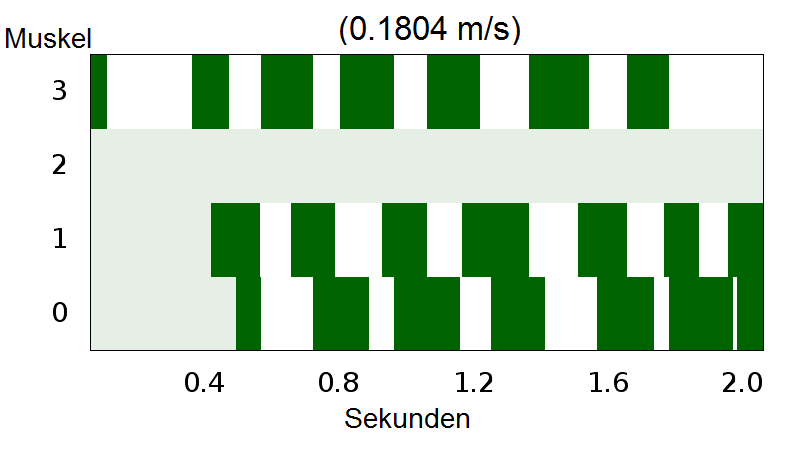
\includegraphics[width=0.9\textwidth]{img/hum26.png}
		\end{figure}
	\end{columns}
\end{frame}

\begin{frame}
	\frametitle{Messergebnisse (5/6)}
	\begin{columns}
		\column{.5\textwidth}
		\begin{figure}
			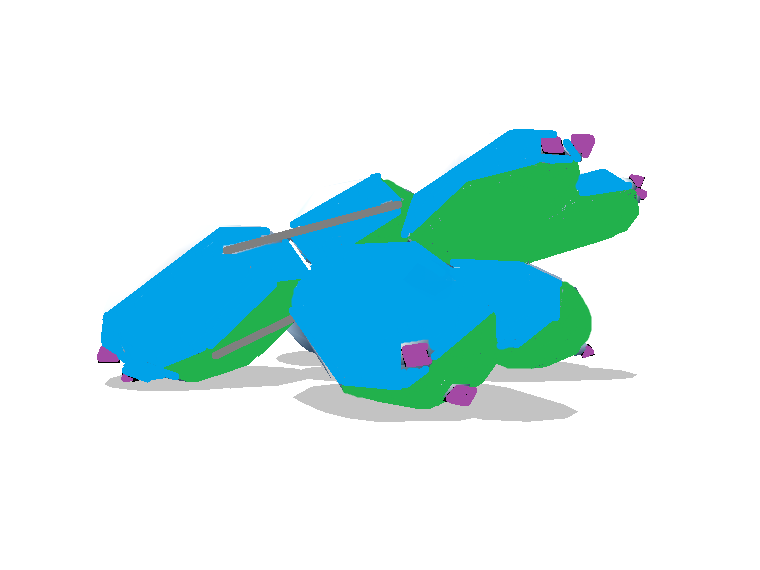
\includegraphics[width=0.68\textwidth]{img/type3.png} \pause 
		\end{figure}
		\begin{figure}
			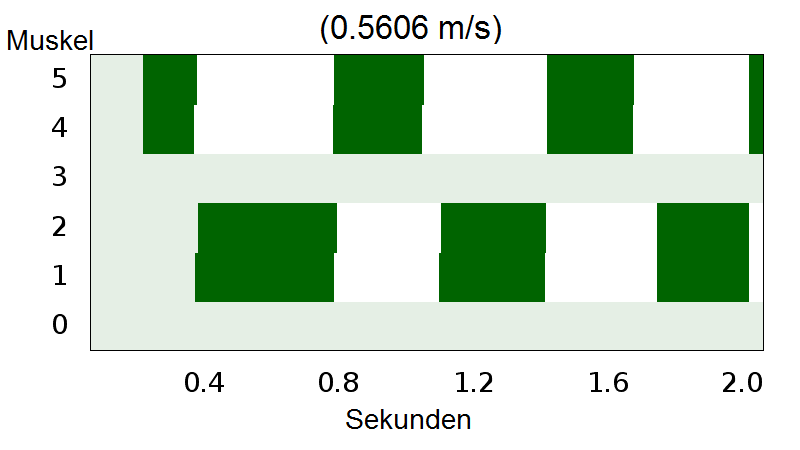
\includegraphics[width=0.9\textwidth]{img/hum32.png}
		\end{figure}
		\column{.5\textwidth}
		\begin{figure}
			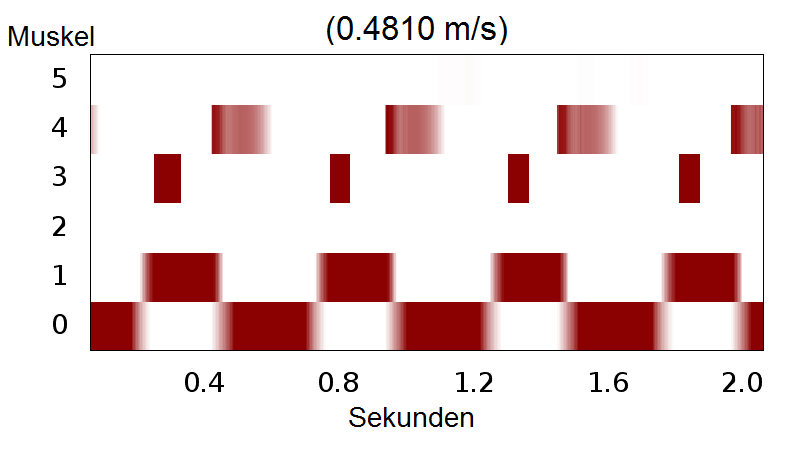
\includegraphics[width=0.9\textwidth]{img/ki3.png} 
		\end{figure}
		\begin{figure}
			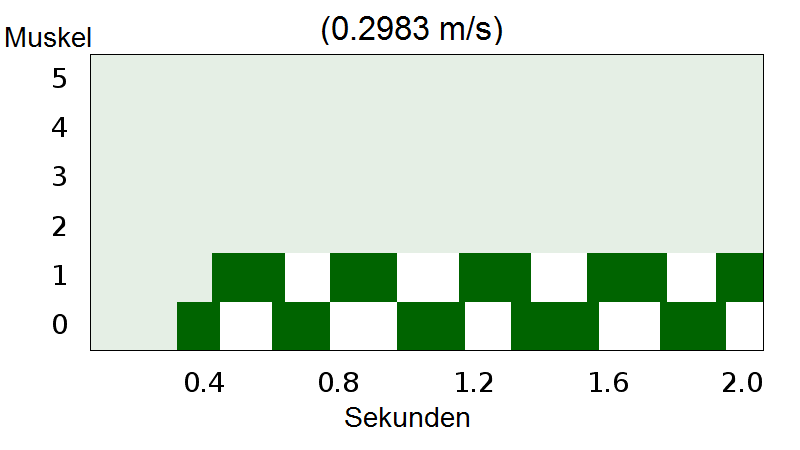
\includegraphics[width=0.9\textwidth]{img/hum31.png}
		\end{figure}
	\end{columns}
\end{frame}

\begin{frame}
	\frametitle{Messergebnisse (6/6)}
	\begin{columns}
		\column{.5\textwidth}
		\begin{figure}
			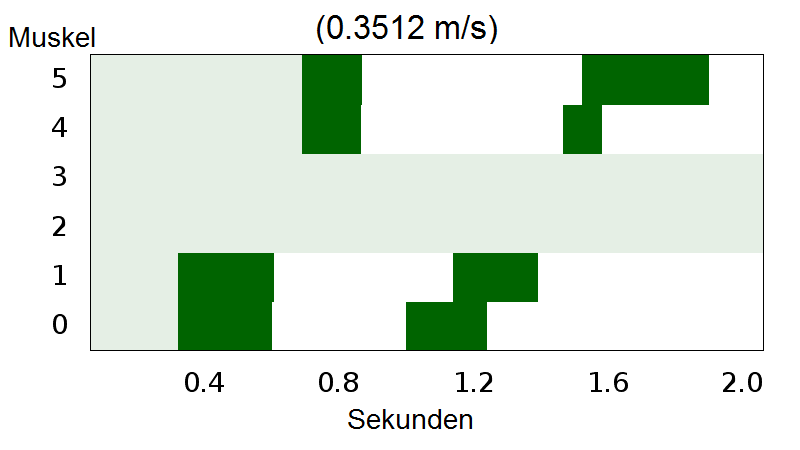
\includegraphics[width=0.9\textwidth]{img/hum33.png} 
		\end{figure}
		\begin{figure}
			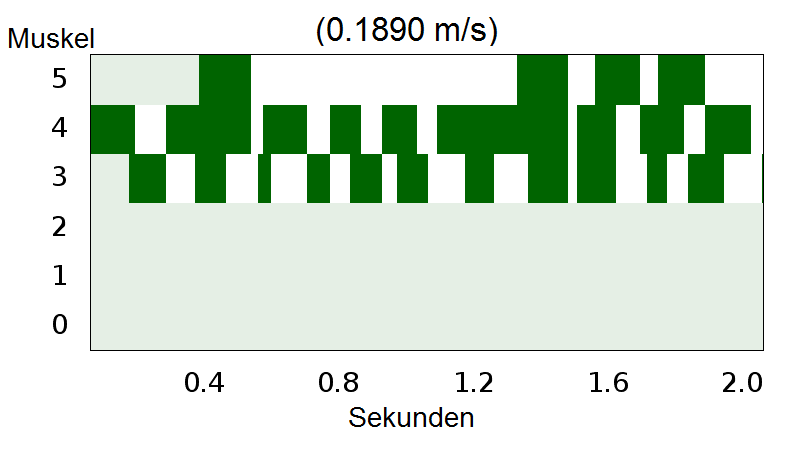
\includegraphics[width=0.9\textwidth]{img/hum35.png}
		\end{figure}
		\column{.5\textwidth}
		\begin{figure}
			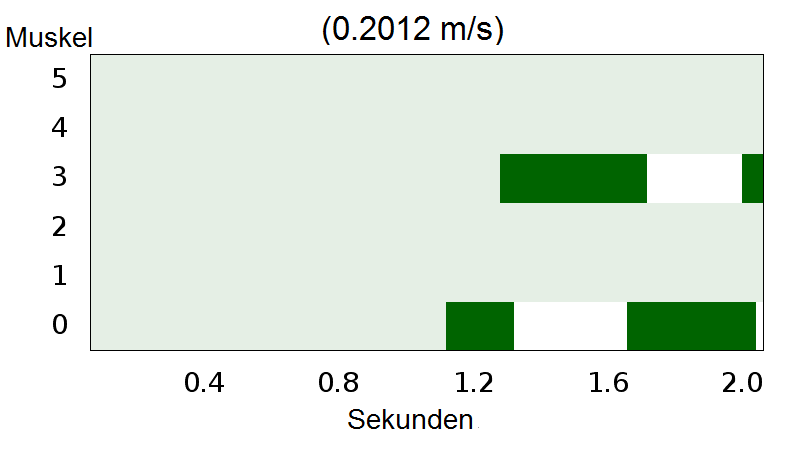
\includegraphics[width=0.9\textwidth]{img/hum34.png} 
		\end{figure}
		\begin{figure}
			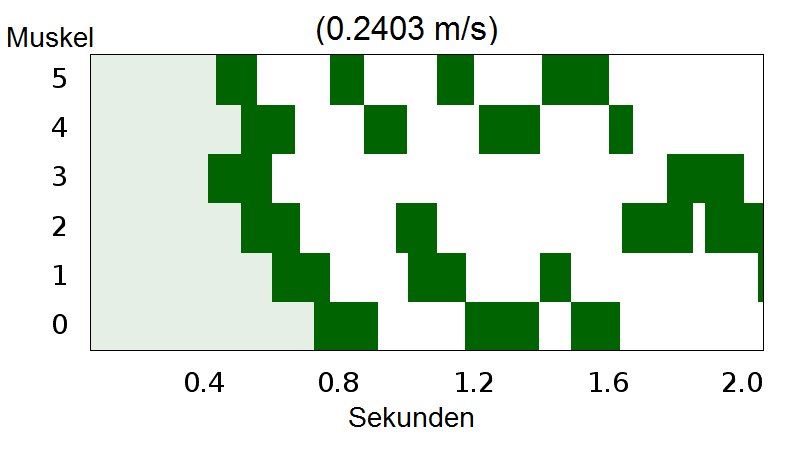
\includegraphics[width=0.9\textwidth]{img/hum36.png}
		\end{figure}
	\end{columns}
\end{frame}

%Ende meiner Folien

\begin{frame}
	\frametitle{Evolutionäre Generierung von Evolved Virtual Creatures}
	Entwickle \textbf{Körperteile + Muskeln + Gehirn} gleichzeitig\\ \pause
	\vspace{2em}
	
	Methode: \textbf{Evolutionärer Algorithmus} \pause
	\begin{enumerate}
		\item Mutation
		\item Reproduktion
		\item Selektion
	\end{enumerate}
	\pause
	\vspace{2em}
	\textbf{Fitness:} Laufgeschwindigkeit \pause  + Ästhetik
\end{frame}

\begin{frame}
	\frametitle{Evolutionäre Generierung von Evolved Virtual Creatures}
	\textbf{Algorithmus}\\
	\vspace{1em}
	
	\begin{itemize}
		\item Starte mit einer Population von 100 zufälligen Kreaturen \\
		\vspace{1em}
		\item In jeder Generation:
		\begin{enumerate}
			\item Messe Fitness
			\item Verwerfe die schlechtesten $80\%$
			\item Fülle Population mit Mutationen oder Nachkommen auf
		\end{enumerate}
		\vspace{1em}
		\item Wiederhole für 500 Generationen\\
	\end{itemize}
	\vspace{2em}
	Ergebnis: Fitness der Population nimmt zu \checkmark
\end{frame}

\begin{frame}
	\frametitle{Evolutionäre Generierung von Evolved Virtual Creatures}
	
	\textbf{Mutation: Zufällige Veränderung einer bestehenden Kreatur}
	\vspace{1em}
	\begin{itemize}
		\item Booleans werden geflippt
		\item Zahlen werden zufällig verschoben (Gauß-verteilt)
		\item Diskrete Werte werden neu gewürfelt
		\item Hinzufügen / Entfernen von Knoten und Kanten
	\end{itemize}
	\vspace{2em}
	Ungenutzte Knoten und Kanten werden gelöscht
\end{frame}

\begin{frame}
	\frametitle{Evolutionäre Generierung von Evolved Virtual Creatures}
	
	\textbf{Paarung: Zufällige Kombination von zwei bestehenden Kreaturen} \\
	\vspace{1em}
	
	\begin{columns}
		\column{.5\textwidth}
			\centering
			\resizebox{0.9\textwidth}{!}{
				\begin{tikzpicture}[->,shorten >=1pt,auto,node distance=0.8cm,main node/.style={circle,draw,font=\sffamily\Large\bfseries}]
				
				\node[main node] (1) {};
				\node[main node] (2) [right of = 1] {};
				\node[main node] (3) [right of = 2] {};
				\node[main node] (4) [right of = 3] {};
				\node[main node] (5) [right of = 4] {};
				
				\path[] (1) edge [bend left = 40] node[left] {} (2);
				\path[] (1) edge [bend left = 80] node[left] {} (3);
				\path[] (3) edge [bend left = 30] node[left] {} (4);
				\path[] (3) edge [bend left = 60] node[left] {} (4);
				\path[] (4) edge [bend left = 40] node[left] {} (5);
				
				\draw (3) to [out=120,in=70,looseness=8] (3);
				
				\end{tikzpicture}
			}
		\column{.5\textwidth}
			\centering
			\resizebox{0.7\textwidth}{!}{
				\begin{tikzpicture}[->,shorten >=1pt,auto,node distance=0.8cm,main node/.style={circle,draw,font=\sffamily\Large\bfseries}]
				
				\node[main node] (1) {};
				\node[main node] (2) [right of = 1] {};
				\node[main node] (3) [right of = 2] {};
				\node[main node] (4) [right of = 3] {};
				
				\path[] (1) edge [bend left = 10] node[left] {} (2);
				\path[] (1) edge [bend left = 30] node[left] {} (2);
				\path[] (1) edge [bend left = 50] node[left] {} (2);
				\path[] (1) edge [bend left = 50] node[left] {} (2);
				\path[] (2) edge [bend left = 30] node[left] {} (3);
				\path[] (2) edge [bend left = 60] node[left] {} (4);
				
				\draw (4) to [out=110,in=70,looseness=8] (4);
				
				\end{tikzpicture}
			}			
	\end{columns}
	
	\vspace{0.6em}
	
	\begin{center}
		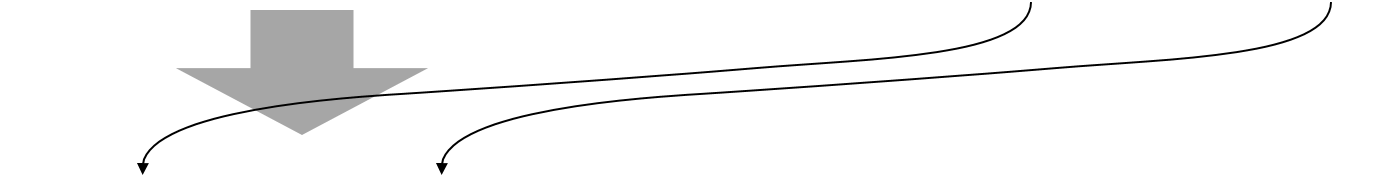
\includegraphics[width=0.9\textwidth]{img/pfeile.png}
	\end{center}
	
	
	\resizebox{0.46\textwidth}{!}{
		\begin{tikzpicture}[->,shorten >=1pt,auto,node distance=0.8cm,main node/.style={circle,draw,font=\sffamily\tiny\bfseries}]
		
		\node[main node] (1) {};
		\node[main node] (2) [right of = 1] {};
		\node[main node] (3) [right of = 2] {};
		\node[main node] (4) [right of = 3] {};
		\node[main node] (5) [right of = 4] {};
		
		\path[] (1) edge [bend left = 40] node[left] {} (2);
		\path[] (1) edge [bend left = 80] node[left] {} (3);
		\path[] (3) edge [bend left = 30] node[left] {} (4);
		\path[] (3) edge [bend left = 60] node[left] {} (4);
		
		\path[] (2) edge [bend left = 30] node[left] {} (3);
		\path[] (2) edge [bend left = 60] node[left] {} (4);
		
		\draw (4) to [out=110,in=70,looseness=8] (4);
		
		\end{tikzpicture}
	}
	
	\vspace{1em}	
	\textbf{Methode A}: Nehme Knoten eines Elternteils und erstetze zufällige Knoten durch die des anderen Elternteils an der gleichen Position
	\vspace{2em}
\end{frame}

\begin{frame}
	\frametitle{Evolutionäre Generierung von Evolved Virtual Creatures}
	
	\textbf{Paarung: Zufällige Kombination von zwei bestehenden Kreaturen} \\
		\vspace{1em}
		
		\begin{columns}
			\column{.5\textwidth}
			\centering
			\resizebox{0.9\textwidth}{!}{
				\begin{tikzpicture}[->,shorten >=1pt,auto,node distance=0.8cm,main node/.style={circle,draw,font=\sffamily\Large\bfseries}]
				
				\node[main node] (1) {};
				\node[main node] (2) [right of = 1] {};
				\node[main node] (3) [right of = 2] {};
				\node[main node] (4) [right of = 3] {};
				\node[main node] (5) [right of = 4] {};
				
				\path[] (1) edge [bend left = 40] node[left] {} (2);
				\path[] (1) edge [bend left = 80] node[left] {} (3);
				\path[] (3) edge [bend left = 30] node[left] {} (4);
				\path[] (3) edge [bend left = 60] node[left] {} (4);
				\path[] (4) edge [bend left = 40] node[left] {} (5);
				
				\draw (3) to [out=120,in=70,looseness=8] (3);
				
				\end{tikzpicture}
			}
			\column{.5\textwidth}
			\centering
			\resizebox{0.7\textwidth}{!}{
				\begin{tikzpicture}[->,shorten >=1pt,auto,node distance=0.8cm,main node/.style={circle,draw,font=\sffamily\Large\bfseries}]
				
				\node[main node] (1) {};
				\node[main node] (2) [right of = 1] {};
				\node[main node] (3) [right of = 2] {};
				\node[main node] (4) [right of = 3] {};
				
				\path[] (1) edge [bend left = 10] node[left] {} (2);
				\path[] (1) edge [bend left = 30] node[left] {} (2);
				\path[] (1) edge [bend left = 50] node[left] {} (2);
				\path[] (1) edge [bend left = 50] node[left] {} (2);
				\path[] (2) edge [bend left = 30] node[left] {} (3);
				\path[] (2) edge [bend left = 60] node[left] {} (4);
				
				\draw (4) to [out=110,in=70,looseness=8] (4);				
				\end{tikzpicture}
			}			
		\end{columns}
		
		\vspace{0.4em}
		
		\begin{center}
			
\includegraphics[width=0.35\textwidth]{img/pfeile2.png}
		\end{center}
		
		\begin{center}
			\resizebox{0.8\textwidth}{!}{
				\begin{tikzpicture}[->,shorten >=1pt,auto,node distance=0.8cm,main node/.style={circle,draw,font=\sffamily\tiny\bfseries}]
				
				\node[main node] (1) {};
				\node[main node] (2) [right of = 1] {};
				\node[main node] (3) [right of = 2] {};
				\node[main node] (4) [right of = 3] {};
				\node[main node] (5) [right of = 4] {};
				\node[main node] (6) [right of = 5] {};
				\node[main node] (7) [right of = 6] {};
				\node[main node] (8) [right of = 7] {};
				\node[main node] (9) [right of = 8] {};
				
				\path[] (1) edge [bend left = 40] node[left] {} (2);
				\path[] (1) edge [bend left = 80] node[left] {} (3);
				\path[] (3) edge [bend left = 30] node[left] {} (4);
				\path[] (3) edge [bend left = 60] node[left] {} (4);
				\path[] (4) edge [bend left = 40] node[left] {} (5);
				
				\draw (3) to [out=120,in=70,looseness=8] (3);
				
				\path[] (6) edge [bend left = 10] node[left] {} (7);
				\path[] (6) edge [bend left = 30] node[left] {} (7);
				\path[] (6) edge [bend left = 50] node[left] {} (7);
				\path[] (6) edge [bend left = 50] node[left] {} (7);
				\path[] (7) edge [bend left = 30] node[left] {} (8);
				\path[] (7) edge [bend left = 60] node[left] {} (9);
				
				\draw (9) to [out=110,in=70,looseness=8] (9);
				
				\path[] (4) edge [bend left = 60] node[left] {} (7);				
				\end{tikzpicture}
			}		
		\end{center}
		
		\vspace{0.6em}	
		
	\textbf{Methode B}: Konkateniere beide Listen und "verknote" Kanten zwischen beiden Teilen
\end{frame}

\begin{frame}
	\frametitle{Evolutionäre Generierung von Evolved Virtual Creatures}
	
	\textbf{Evolution in der Praxis}
	\begin{itemize}
		\item Physiksimulation zur Berechnung jeder Fitnessfunktion notwendig
		\item Parallele Berechnung
		\item Optimierung: Breche Simulationen ab, die keinen Erfolg versprechen
		\item Rundungsfehler, Bugs, Energie-Leaks werden gefunden und ausgenutzt
		\item Verhindere triviale Lösungen (Umfallen)
	\end{itemize}
\end{frame}

\begin{frame}
	\frametitle{Beispiele von EVCs}
	
	TODO Marian
\end{frame}


\begin{frame}
	\frametitle{Spielmechanik}
	
	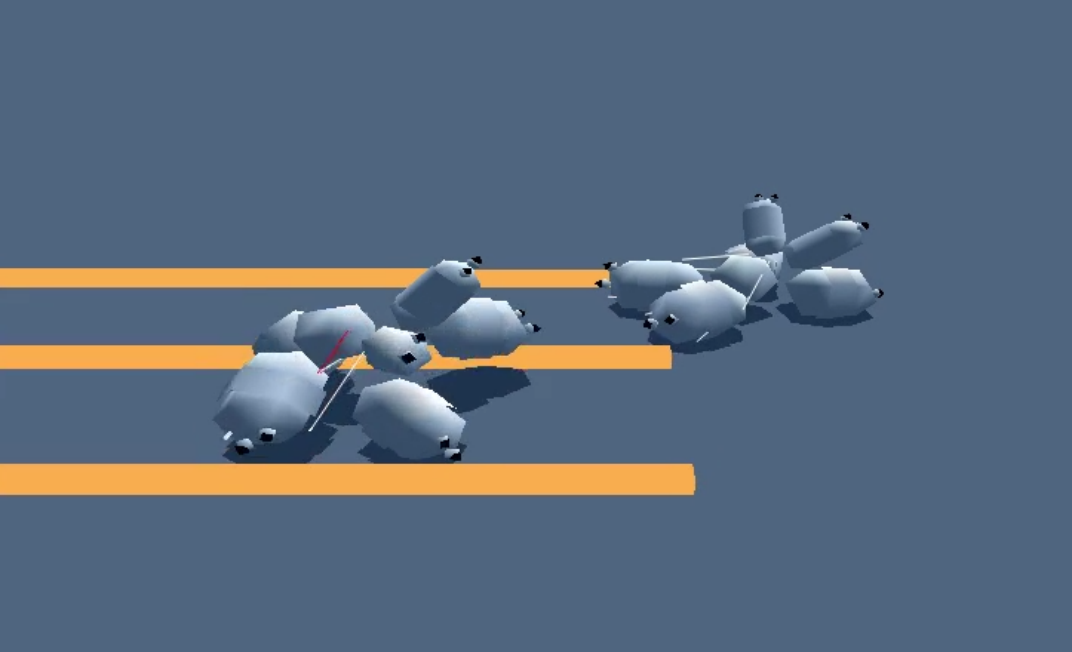
\includegraphics[width=0.5\textwidth]{img/games/darwin.png}
	\vspace{1em}
	
	\textbf{Ablauf}: Mensch und Computer steuern Kopien der gleichen Kreatur \\
	\vspace{1em}
	\textbf{Mensch}: Taste für jeden Muskel \\
	\textbf{Computer}: Generiertes Gehirn \\
	\vspace{1em}
	\textbf{Spielende}: Beide erreichen das Ziel \textbf{oder} Zeit läuft ab \\
	\vspace{1em}
	Mensch und Computer haben unterschiedliche Sensoren und Aktoren.
\end{frame}

\begin{frame}
	\frametitle{Auswertung der Playtests}
	
	TODO Christopher
\end{frame}


\begin{frame}
	\frametitle{Mögliche Erweiterungen}
	
	\textbf{Ziele}:\\ Springen, Schwimmen, Kämpfen, Klettern... \\
	\vspace{2em}
	\textbf{Spielmechaniken}:\\ Sammeln und Tauschen von Kreaturen, Online-Multiplayer \\
	\vspace{2em}
	\textbf{Fairness}:\\ Binäre Eingaben für Computer
\end{frame}

\begin{frame}
	\frametitle{Zusammenfassung}
	\pause
	\textbf{Vorgehensweise}
	\begin{itemize}
		\item Körper und Gehirn werden gemeinsam entwickelt \pause
		\item Ersetze evolutionäres Gehirn durch menschlichen Spieler \pause
	\end{itemize}
	\vspace{1em}
	\textbf{Ergebnis}
	\begin{itemize}
		\item Tragfähiges, erweiterbares Spielkonzept \pause
		\item Menschen sind evolutionärem Gehirn unterlegen \pause
	\end{itemize}
	\vspace{1em}
	\begin{block}{Take Home Message}
		Evolutionäre virtuelle Kreaturen sind interessante Spielgegenstände. Sie können allerdings nicht in Echtzeit generiert werden.
	\end{block}
	
\end{frame}

\end{document} 